% =============================================================================================
% Calibrating first-principles lattice thermal conductivity to experiment:
% a curated half-Heusler dataset and a validated transfer function
%
% Target journal: Computational Materials Science (Elsevier), elsarticle class.
%
% TO COMPILE (Overleaf: upload this folder, set manuscript.tex as the main document):
%     pdflatex manuscript  ->  bibtex manuscript  ->  pdflatex x2
%
% BEFORE SUBMITTING, run both gates from the repository root:
%     python make_paper_numbers.py           regenerates every figure quoted in the text
%     python verify_citations.py paper/manuscript.tex
% The second fails on an undefined citation key, a DOI that no longer resolves, or a citation
% with no recorded supporting sentence in claims_ledger.csv. All three are blocking.
%
% Authors and affiliations are set. ORCIDs: Shivam Randive and Himanshu Pandey are recorded in
% the frontmatter comment; Ojaswini Randive's is still awaited.
% =============================================================================================

% `authoryear` puts natbib in author-year mode, which contradicts \bibliographystyle{elsarticle-num}
% below and renders the citations malformed. Every citation in this manuscript is a plain \cite --
% there is no \citep or \citet anywhere -- so the numeric style is the one we want and the class
% option is what has to go.
\documentclass[preprint, 12pt]{elsarticle}

\usepackage[T1]{fontenc}
\usepackage[utf8]{inputenc}      % author names carry o-slash, s-caron, l-stroke etc.
\usepackage{amsmath, amssymb}
\usepackage{graphicx}
\usepackage{booktabs}
\usepackage[separate-uncertainty=true, detect-weight=true]{siunitx}
\usepackage[version=4]{mhchem}
\usepackage{microtype}
\usepackage[hidelinks]{hyperref}

% Half Heuslers are written as \ce{ZrNiSn}; keep chemistry upright inside bold table cells.
\sisetup{group-separator = {,}, group-minimum-digits = 4}

% =============================================================================================
% WHAT MUST STILL BE FILLED IN BEFORE SUBMISSION (two items).
% Both are rendered into the PDF, so each is defined here rather than left inline where it
% can be missed. check_tex_structure.py fails the build while any of them still says TO BE ADDED.
% =============================================================================================
% Authors are Shivam Randive (corresponding), Himanshu Pandey, Ojaswini Randive -- set in the
% frontmatter below. Two things about that block still need confirming:
%   1. The \ead is i22ph019@phy.svnit.ac.in, which is what this repository was worked from. It is
%      attached to Shivam Randive as corresponding author. Confirm the address belongs to him.
%   2. Ojaswini Randive's affiliation is unknown here and must not be guessed.
\newcommand{\pandeyemail}{PROF. PANDEY EMAIL --- TO BE ADDED}
\newcommand{\repourl}{\texttt{[REPOSITORY URL AND DOI --- TO BE ADDED]}}
% Draft. Confirm the Google credit programme's exact name before submission -- funders and credit
% schemes usually specify the wording they want to be acknowledged by, and getting it wrong is
% worse than omitting it. Add any departmental or institutional support Prof. Pandey advises.
\newcommand{\acknowledgementtext}{%
  Corpus construction used Google Cloud credits, which funded the large-language-model extraction
  of measurements from primary publications described in Section~\ref{sec:dataset}. We thank the
  maintainers of the databases this work rests on---Starrydata2, AFLOW, the Materials Project,
  JARVIS, OQMD, the Crystallography Open Database and the OPTIMADE consortium---whose curation
  made an experiment-anchored corpus of this kind possible, and the authors of the \num{198}
  experimental and \num{22} computational studies whose measurements and calculations are analysed
  here.}

\journal{Computational Materials Science}

\begin{document}

\begin{frontmatter}

\title{Calibrating first-principles lattice thermal conductivity to experiment:
       a curated half-Heusler dataset and a validated transfer function}

% Author order follows the convention of the field: first author did the work, last author is the
% senior/supervising author, middle authors contributed in between. The last position is the
% SECOND most senior, not the least -- putting the supervisor in the middle of a three-author list
% would place him in the weakest slot and imply the third author supervised the project.
% Confirm this order with Prof. Pandey before submission; some departments prefer otherwise.
% ORCID iDs are supplied to Elsevier through Editorial Manager at submission, not through the
% .tex -- elsarticle has no \orcid macro and the publisher adds the iD badges from the submission
% record. Kept here so they are not lost:
%   Shivam Randive    0009-0005-1403-4484   (checksum verified)
%   Ojaswini Randive  awaiting
%   Himanshu Pandey   0000-0002-7380-366X   (checksum verified)
\author[svnit]{Shivam Randive\corref{cor1}}
\ead{i22ph019@phy.svnit.ac.in}
\author[nitrr]{Ojaswini Randive}
\author[svnit]{Himanshu Pandey\corref{cor1}}
\ead{\pandeyemail}
\cortext[cor1]{Corresponding authors.}

\affiliation[svnit]{organization={Department of Physics, Sardar Vallabhbhai National Institute
                                  of Technology},
                    city={Surat},
                    country={India}}
% Confirm the department's exact official name against the NIT Raipur website before submission:
% affiliations are indexed verbatim by Scopus and Web of Science, so a paraphrase can detach the
% paper from the institution's record.
\affiliation[nitrr]{organization={Department of Metallurgical and Materials Engineering,
                                  National Institute of Technology Raipur},
                    city={Raipur},
                    state={Chhattisgarh},
                    country={India}}

% =============================================================================================
% ABSTRACT + KEYWORDS.  Draft 2 -- reordered after review.
%
% Draft 1 opened with a deficiency in other people's models and reached our own contribution in
% sentence three; the number that matters landed in sentence five of six. It also quoted our
% 86.8% within-2x without the null's 78.9%, which on 38 compounds is a three-compound gap -- the
% body states this plainly and the abstract did not, so the abstract was the least honest part of
% the paper.
%
% Draft 2 leads with the resource, then the measured offset, then the correction, and quotes the
% null beside our own figure. The rank correlation -- the statistically robust result -- is now
% stated rather than buried.
%
% Draft 3 (2026-09-04): the closing sentence named only the issued five and the eleven declined,
% so a reader of the abstract alone could not tell the ten conditional estimates existed -- and
% the roadmap they carry ("two measurements in Ni-Bi release nine predictions") is one of the
% paper's distinctive contributions. Now all three tiers are named.
%
% 222 words. No number here that is not also in the body and in paper_numbers.json.
% =============================================================================================

\begin{abstract}
Lattice thermal conductivity governs thermoelectric performance, yet for half-Heusler compounds it
has been measured for only about fifty materials while being calculated for hundreds. We assemble
what is, to our knowledge, a near-exhaustive corpus of the measured values: \num{52} half Heuslers
drawn from \num{164} publications, alongside \num{289} with full Boltzmann-transport calculations,
in which every value carries an explicit provenance and method tier so that measurements and
calculations are never pooled. The corpus shows that the two disagree systematically: published
calculations exceed measured $\kappa_L$ by a median factor of \num{1.55}. Models trained and
validated on calculated labels, which is standard in this field, therefore predict a quantity that
differs from the experiment they are meant to guide. We fit a two-parameter transfer function
mapping calculation onto measurement, and evaluate it with each compound's entire chemistry
withheld from both the model and the calibration. Within a domain fixed in advance---semiconducting,
cubic, non-polymorphic---it achieves \SI{33.7}{\percent} median error, averaged over five model seeds, against \SI{50.5}{\percent}
for the same model output uncorrected and \SI{94.6}{\percent} for published semi-empirical estimates, and
ranks compounds with Spearman $\rho=\num{0.65}$. It places \SI{86.8}{\percent}
of compounds within a factor of two, against \SI{78.9}{\percent} for a compound-blind baseline.
We issue five predictions, decline eleven with the criterion each fails, and report ten further
estimates as conditional, naming the measurement that would qualify each.
\end{abstract}

\begin{keyword}
half-Heusler \sep lattice thermal conductivity \sep thermoelectric materials \sep
Boltzmann transport \sep experimental validation \sep materials data
\end{keyword}


\end{frontmatter}

% =============================================================================================
% SECTION 1 -- INTRODUCTION.  Draft 2 -- rebuilt on the six-block structure of Paliwal & Alam
% (arXiv:2511.13202v3), which this manuscript follows throughout.
%
% Seven paragraphs, one job each:
%   1 why the property matters          2 the computational route and its cost
%   3 the mismatch, quantified          4 THE GAP -- prior work named, then one shared criticism
%   5 the scarcity that makes it hard   6 what we did, in paper order
%   7 the contrast claim
%
% Draft 1 buried the gap across paragraphs 3, 6 and 7, opened the differentiation defensively
% ("We are not the first to bridge the two scales"), and ended four times over: a numbered
% contributions list, a strategy paragraph, and a pre-emptive disclaimer. The disclaimer moved to
% the Limitations subsection where it can be quantified; the list became prose.
%
% Every citation here was resolved through Crossref from a real search and carries a row in
% claims_ledger.csv. None was written from memory.
% =============================================================================================

\section{Introduction}
\label{sec:intro}

A thermoelectric generator asks one material to carry charge freely and to obstruct heat at the
same time, and half Heuslers are unusually good at the first half of that bargain and unusually
poor at the second. They are mechanically robust, stable to high temperature, and built from
abundant, non-toxic elements; figures of merit approaching $zT \approx 1.5$ have been demonstrated
in $p$-type \ce{FeNbSb}~\cite{fu2015realizing} and $zT \approx 1.4$ in
\ce{ZrCoBi}~\cite{zhu2018discovery}. What holds the class back is that it conducts heat through the
lattice too well. Because the figure of merit varies inversely with the lattice thermal
conductivity $\kappa_L$, essentially every advance in this family has come from suppressing it.
Identifying compounds whose $\kappa_L$ is intrinsically low is therefore the central screening
problem, and it is the one this paper addresses.

In principle that screen can be run without entering a laboratory. Solving the phonon Boltzmann
transport equation from first principles yields $\kappa_L$ with no experimental input, and the
method has been applied across the half-Heusler space to pick out compounds of unusually low
conductivity~\cite{carrete2014finding}. The obstacle is cost. A converged calculation is expensive
enough that exhaustive enumeration is impractical, and a great deal of effort has consequently gone
into reproducing the calculation more cheaply---through compressed-sensing
descriptors~\cite{liu2020a} and, increasingly, through machine-learned models trained on databases
of computed
conductivities~\cite{luo2023predicting,trans2022lattice,miyazaki2021machine,jaafreh2021lattice,bhattacharjee2022thorough,paliwal2025accelerate}.
Those models are fast, and they are accurate against the quantity they were trained on.

That quantity is not the one a laboratory measures. Models in this line are trained on
\emph{calculated} labels because calculated labels are what exist in quantity, so their reported
accuracies are accuracies against calculation; no claim is made in those papers that the output is
a measurement, but the inference is left to the reader and the reader makes it. It does not hold.
In the corpus assembled for this work, published transport calculations exceed the measured lattice
thermal conductivity of the same compound by a median factor of \num{1.55}. A model reproducing
calculations to \SI{10}{\percent} is therefore roughly \SI{55}{\percent} away from the experiment it
exists to guide. That calculated $\kappa_L$ runs high is not itself news---it is documented compound
by compound throughout the half-Heusler literature, and attacked compound by compound by
identifying the responsible defect chemistry. What has not been available is the size of the offset
across a class, and a correction for it validated against held-out experiment.

Three routes across that gap already exist, and the differences between them matter. Zhu
\emph{et al.} trained a crystal-graph neural network on \num{2668} computed conductivities and
transfer-learned it onto \num{132} experimentally measured values, roughly halving the error on the
measured scale; the computed labels they began from were themselves semi-empirical estimates rather
than transport calculations~\cite{zhu2021charting}. Miller \emph{et al.} fitted the parameters of a
semi-empirical Umklapp model directly to experimental data~\cite{miller2017capturing}. Chen
\emph{et al.} bypassed calculation altogether, training a Gaussian-process model on the measured
conductivities of about one hundred inorganic solids~\cite{chen2019machine}. In none of these is the
object being corrected a full Boltzmann-transport calculation. The distinction is not cosmetic:
semi-empirical and transport-calculated conductivities for the same compound differ by a median
factor of \num{1.38} with a tail to \num{7.2} (Section~\ref{sec:tiering}), so they are different
inputs and require different corrections.

Correcting a transport calculation requires measurements to correct it against, and here the
imbalance is severe. Of the \num{742} half Heuslers in our corpus carrying a thermal conductivity
record of any kind, \num{289} have a full transport calculation and \num{52} have ever been measured
in a laboratory---a ratio of \num{5.6} to one. Training a model directly on measurements is the
obvious alternative and is beginning to appear~\cite{barua2024interpreta}, but \num{52} compounds
are too few to learn a structure--property relation from scratch. They are, as we show, enough to
calibrate one.

This paper therefore takes the opposite route to the usual one. Rather than train a model to
reproduce calculations more cheaply, we take the calculations as given and ask what it costs to move
them onto the experimental scale. We assemble an experiment-anchored corpus---\num{52} measured
compounds drawn from \num{164} publications alongside \num{289} carrying transport calculations,
every value tagged with its provenance and an explicit method tier so that measurements and
calculations are never pooled (Section~\ref{sec:dataset}). We measure the offset between the two
scales and fit a two-parameter transfer function that removes it
(Section~\ref{sec:transfer}). We then validate that function with each compound's entire chemistry
withheld from the calibration as well as from the model: inside a domain of applicability declared
in advance, the corrected predictions place \SI{86.8}{\percent} of \num{38} held-out compounds
within a factor of two of measurement at \SI{33.7}{\percent} median error, against
\SI{50.5}{\percent} median error uncorrected and \SI{44.0}{\percent} for the better of two
compound-blind nulls given the same holdout (Section~\ref{sec:blind}). On that basis we issue five
predictions for unmeasured compounds, each with a measured-coverage interval, and decline eleven
further candidates, naming the condition each fails (Sections~\ref{sec:issued}
and~\ref{sec:refusals}). Five modifications to the method were implemented and rejected on held-out
evidence, including one whose premise the data support but whose benefit does not transfer; we
report those alongside the result they failed to improve (Section~\ref{sec:rejected}).

What separates this from the existing routes is the object being corrected and the form of the
correction. The object is the transport calculation itself rather than a semi-empirical proxy for
it. The correction is closed-form---two parameters a reader can apply by hand and interrogate
physically, not a fitted network---and it carries a domain of applicability that was declared
before the validation set was scored and is tested rather than asserted. The result is not a cheaper
calculation. It is a calculation moved onto the scale on which experiments are reported.

% =============================================================================================
% SECTION 2 -- METHODS.  Draft 2 -- merge of the former Section 2 (Dataset) and Section 3 (Method).
%
% Two structural faults in the split version are fixed here:
%
%   1. The transfer function -- the substantive contribution -- was 487 words and sat AFTER the
%      816-word regression-model subsection that the deployed route does not even use. The order
%      is now contribution first, auxiliary component second, and the auxiliary subsection is
%      titled for what it actually is ("Supplying a calculation where none exists").
%
%   2. The tier list reported 505 under a definition that only 289 compounds satisfy. 505 is the
%      database's first-principles flag; 289 is the stricter method-string match. Both numbers are
%      correct and are now presented as the refinement they are, with the 214 + 2 remainder.
%
% Statements that appeared twice in the split version are stated once here: the TiNiSn/ZrNiSn row
% imbalance (was in 3.3 and again in 3.5), the fit-objective rule (3.3 and 3.5), and the
% held-out-nulls principle (3.5, 3.6 and twice more in Results).
%
% All labels from the split sections are preserved so existing \ref calls still resolve.
% =============================================================================================

\section{Methods}
\label{sec:method}

We want the \emph{measured} lattice thermal conductivity of a half Heusler, and we obtain it in two
steps: a transfer function that maps a first-principles value onto the experimental scale, and,
only where no calculation exists, a regression model that supplies the first-principles value
itself. The transfer function is the substantive contribution and is described first.
Figure~\ref{fig:method} shows the whole procedure together with the property that organises it.
Measurements and calculations run in separate tracks from the corpus onward and meet only at the
transfer function, so nothing fitted to a calculation is ever scored against another calculation.

\begin{figure}[tb]
  \centering
  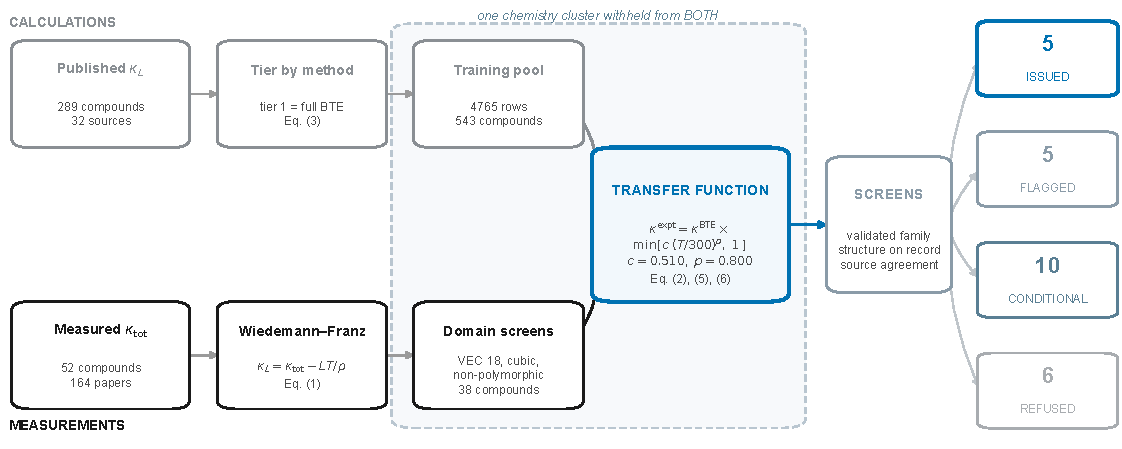
\includegraphics[width=\linewidth]{figures/fig08_method.pdf}
  \caption{\textbf{The method, end to end.} Calculations (upper track) and measurements (lower
  track) are never pooled: they are tiered, filtered and counted separately and meet only at the
  transfer function, which is the sole point at which a calculated quantity is mapped onto an
  experimental one. The dashed region marks what a fold of the validation removes---an entire
  chemistry cluster, withheld from the regression model \emph{and} from the calibration, since
  holding one out but not the other would let the transfer function see the compound it is being
  scored on. Counts are the funnel from \num{289} published calculations and \num{52} measured
  compounds down to the five issued predictions; equation numbers refer to
  Section~\ref{sec:method}.}
  \label{fig:method}
\end{figure}

\subsection{Corpus construction}
\label{sec:dataset}
\label{sec:sources}
\label{sec:composition}

A correction between calculation and experiment can only be fitted where both exist for the same
compound, so the first requirement is a corpus in which the two are separately identifiable. Ours
contains \num{967} distinct compounds, of which \num{742} are half Heuslers, drawn from \num{211}
publications and structure repositories---\num{7823} temperature-resolved values across the
half-Heusler subset---and every value carries its provenance and a statement of how it was
obtained.

Experimental values come from the Starrydata curated transport
database~\cite{katsura2025starrydata}, read at the published snapshot of 1 July
2025~\cite{mato2025starrydata}, from direct extraction of primary publications, and from targeted
recovery of measurements that existed in our own extraction records but had never reached the
training table. The two Starrydata citations are the resource and the dated version actually used,
so the corpus can be regenerated exactly. Starrydata supplies \SI{95}{\percent} of the experimental
rows, and those rows trace to \num{150} distinct primary publications, since it aggregates
digitised transport curves and does not measure anything itself. Seven compounds
(\ce{AlNiSb}, \ce{AlVNi}, \ce{DySbPt}, \ce{LuSbPt}, \ce{TbSbPt}, \ce{VNiSn}, \ce{ZrSbIr}) enter
only through direct extraction, and three of them---the \ce{Sb}--\ce{Pt} series members---validate
a bonding family in which we later issue predictions.

Direct extraction from primary publications was performed by a multimodal large language model
(Google Gemini) reading the full text, tables and figures. The method is
productive but not trustworthy on its own, and one failure mode is worth recording because it is
invisible without an explicit check. A publisher's full-text endpoint may return a metadata stub
carrying only a title and a link, and return it with an HTTP success code; \num{167} such stubs were
stored as though they were articles. Given a title alone the model does not decline. It returns
fluent and specific measurements---instrument models, sample densities, figure numbers, whole
temperature series---that are entirely fabricated. Extraction of \num{45} of those stubs produced
\num{1571} invented measurements, of which \num{524} thermal-conductivity rows reached the export
and accounted for \SI{17.4}{\percent} of it before the defect was found. Two safeguards follow.
Extraction is now gated on the retrieved source exceeding \num{3000} bytes, an order of magnitude
below the smallest genuine article body and above the largest observed stub, so a title-only record
is never sent to the model; and affected rows are flagged in place and excluded downstream rather
than deleted, so the contamination remains auditable. Every surviving value must additionally pass
the physical and provenance gates below, which are enforced in code. No
value enters the corpus on the model's authority alone.

First-principles values were drawn from
AFLOW---transport values from its AAPL module~\cite{plata2017an} and quasi-harmonic estimates from
AGL~\cite{toher2014highthroug}, which the tiering below keeps apart---the Materials
Project~\cite{jain2013commentary}, JARVIS~\cite{choudhary2020the}, OQMD~\cite{kirklin2015the} and
published phonon-transport studies. Crystal structures were taken from the same repositories
together with COD and OPTIMADE-federated sources~\cite{andersen2021optimade}.

Experiments measure total thermal conductivity, so the lattice component must be separated from the
electronic one. We do this by Wiedemann--Franz subtraction,
%
\begin{equation}
  \kappa_L = \kappa_\mathrm{tot} - \frac{L T}{\rho},
  \label{eq:wf}
\end{equation}
%
with the Lorenz number $L$ taken from the single-parabolic-band parameterisation of Kim and
Snyder~\cite{kim2015characteri}, $L = 1.5 + \exp(-|S|/116)$ in units of
\SI{1e-8}{\watt\ohm\per\kelvin\squared} with the Seebeck coefficient $S$ in
\si{\micro\volt\per\kelvin}. \SI{85}{\percent} of the experimental rows are obtained this way; the
remainder are reported as lattice conductivity directly. Equation~\eqref{eq:wf} is a difference of
two measured quantities and is only as trustworthy as the resistivity entering it, so we require
$\rho$ to lie in \SIrange{1e-8}{1e-2}{\ohm\meter}, the range physically available to a dense
intermetallic. Rows carrying $\rho$ of order \SI{10}{\ohm\meter}---six orders of magnitude too
large---drive $LT/\rho$ to zero, so the subtraction removes nothing and the row ships the
\emph{total} conductivity under a lattice label. The failure is silent, and its signature is an
apparent lattice conductivity that \emph{rises} with temperature. \num{136} rows failed this gate,
among them all \num{47} rows of \ce{TiCoSn}.

Figure~\ref{fig:corpus} shows what the corpus contains and, equally, what the field contains. Of
the \num{742} half Heuslers with a thermal-conductivity record of any kind, \num{289} carry a
transport calculation and \num{52} have been measured. The measured set is itself unevenly
evidenced: twenty-seven of the \num{52} rest on a single publication, while five have been measured
by ten or more independent groups. We retain both and carry the distinction forward, so that
agreement with a twenty-times-replicated curve is never presented as equivalent to agreement with a
single digitised figure. Overall, Fig.~\ref{fig:corpus} fixes the two facts the rest of the paper
works from: calculations outnumber measurements by \num{5.6} to one, and the measurements rest on
very uneven evidence.

\begin{figure}[tb]
  \centering
  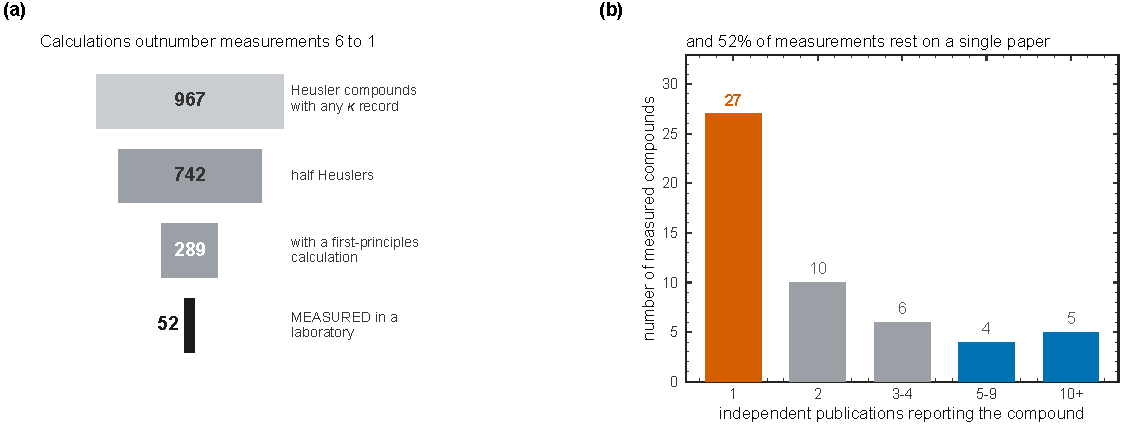
\includegraphics[width=\linewidth]{figures/fig01_corpus.pdf}
  \caption{\textbf{First-principles calculations of half-Heusler lattice thermal conductivity
  outnumber laboratory measurements by \num{5.6} to one.}
  (a) Compounds surviving each stage of corpus construction, drawn to scale. Of \num{967} Heusler
  compounds with a thermal-conductivity record, \num{742} are half Heuslers, \num{289} carry a
  full Boltzmann-transport calculation and \num{52} have been measured.
  (b) Independent publications behind each measured compound. Twenty-seven of \num{52} rest on a
  single source, which sets the evidence tiering used in Section~\ref{sec:results}.}
  \label{fig:corpus}
\end{figure}

\subsection{Method tiering and quality control}
\label{sec:tiering}
\label{sec:gates}

Pooling a measurement with a calculation would destroy the quantity this paper sets out to measure,
so every row carries a \emph{method tier} recording how its value was obtained. Tier~0 is a
laboratory measurement: \num{52} half Heuslers, \num{3482} values, \num{164} publications,
\SIrange{200}{1122}{\kelvin}. Tier~1 is a solution of the phonon Boltzmann transport equation from
third-order force constants. Tier~2 is transport computed on a machine-learned interatomic
potential rather than \emph{ab initio} forces, \num{419} compounds. Tier~3 is a semi-empirical
Slack or Debye--Callaway estimate from elastic and thermodynamic quantities, \num{245} compounds.

For tier~1 the repository flag and the method string disagree. \num{505} half
Heuslers carry a nominally first-principles label, but only \num{289} carry a method string that
positively identifies a transport calculation; \num{214} (\SI{42}{\percent}) carry \emph{only} a
semi-empirical estimate, and two more (\ce{LaSeCl} and \ce{NaSrP}) are labelled merely as an
approximate transport calculation. We assign the tier from the method string and require a positive
match, so that a label we cannot classify counts against us. Throughout this paper tier~1 therefore
means the \num{289}, not the \num{505}.

The two populations are not interchangeable, and the corpus lets us say by how much. For the
\num{93} half Heuslers carrying both kinds of label at a matched temperature, the median
disagreement is a factor of \num{1.38} and \SI{84}{\percent} agree within a factor of two---but the
tail reaches \num{7.2}. The difficulty is dispersion rather than bias: a semi-empirical value is
usually close and occasionally very wrong, and nothing in the value itself indicates which. A
corpus that assigned tiers by repository would average the two and would calibrate a transfer
function partly against values that are themselves fitted estimates.

Five further conditions are enforced in code at the point the corpus is generated, so a rejected
value cannot return when a script is re-run. A compound is admitted as a half Heusler only if a
cubic $C1_b$ record (space group 216) exists in a source that is not a prototype-substitution
database, since prototype decorations record that a structure was \emph{generated}, not that the
phase forms. A compound also recorded in a non-cubic space group is flagged: \ce{MgAgSb} (space
groups 129 and 216) and \ce{DySbPd} (186, 194 and 216) are both dimorphic, and a cubic calculation
cannot be compared to a measurement of a distorted phase without saying so. Half and full Heuslers
are separated by the measured site ratio, not by formula appearance, since a binary in space
group 225 is fluorite, not a Heusler. Values below \SI{200}{\kelvin} are excluded, because the
boundary-free conductivity returned by a transport calculation diverges as $T\to 0$ when Umklapp
scattering freezes out, while the measurement becomes boundary-limited and therefore specific to
the specimen's microstructure; below \SI{200}{\kelvin} the two are not the same quantity. And a
tier-1 row must carry a transport-calculation method string, not a semi-empirical one.

\subsection{The transfer function}
\label{sec:transfer}

A first-principles calculation describes a perfect, infinite crystal, while a laboratory specimen is
a polycrystal with grain boundaries, point defects and finite density, each of which scatters
phonons the calculation allows to propagate freely; for the XNiSn half Heuslers this has been
analysed directly against measurement~\cite{schrade2017the}. The measured conductivity is
accordingly lower, and lower by an amount that grows as the intrinsic phonon mean free path
grows---that is, as temperature falls. We capture this with two parameters,
%
\begin{equation}
  \kappa_L^{\,\mathrm{expt}}(T) \;=\; \kappa_L^{\,\mathrm{BTE}}(T)\;
    \min\!\left[c\left(\frac{T}{300}\right)^{p},\,1\right],
  \label{eq:transfer}
\end{equation}
%
where $c$ sets the room-temperature reduction and $p$ its temperature dependence, and the cap at
unity enforces the physical requirement that extrinsic scattering can only reduce conductivity.
Fitted on the in-domain compounds, $c=\num{0.51}$ and $p=\num{0.80}$. Both are fitted quantities
rather than constants of nature: across leave-one-chemistry-out refits $c$ stays within
\numrange{0.48}{0.51} while $p$ ranges over \numrange{0.80}{1.45}. The suppression at
\SI{300}{\kelvin} is therefore well determined and its temperature dependence is not, and we report
both ranges rather than only the flattering one.

Equation~\eqref{eq:transfer} is not, however, a boundary-scattering model, and the reason is a
bound rather than a preference. A Callaway grey-boundary
treatment~\cite{callaway1959model} with a single boundary length gives a suppression
$S = \Lambda_\mathrm{b}/(\Lambda+\Lambda_\mathrm{b})$ which, with $\Lambda \propto 1/T$, has
logarithmic slope $1-S$ at \SI{300}{\kelvin}---so a boundary model reproducing $S(300)=c$ must have
$p = 1-c$. Generalising to a spectral model, with a per-mode suppression $S_\omega$ and any
distribution of mode conductivities, the slope is
$1 - \langle S^2\rangle_\kappa/\langle S\rangle_\kappa \leq 1-\bar S$ by the Cauchy--Schwarz
inequality. The constraint is therefore not a modelling convenience but a \emph{ceiling}: no
single-boundary-length model, grey or spectral, can produce a slope above $1-c$. At $c=\num{0.51}$
that ceiling is \num{0.49}, and our fitted $p=\num{0.80}$ exceeds it by a factor of \num{1.63}.
Raising the ceiling would require intrinsic mean free paths steeper than
$\Lambda \propto T^{-1.63}$, and the calculations we are correcting do not show that: their own
logarithmic slopes have a median of $-1.00$.

We therefore report the two-parameter form together with the conclusion that follows from it:
\textbf{the correction is not boundary-limited transport}. Its magnitude is of the right order for
grain-boundary scattering in these materials, but its temperature dependence is steeper than that
mechanism alone allows, which implies at least one further temperature-dependent contribution.
Equation~\eqref{eq:transfer} is an empirical transfer function, and we attach no mechanism to its
parameters.

\subsection{What is predicted, and how it is scored}
\label{sec:definitions}

The calculated quantity being calibrated is the phonon Boltzmann-transport conductivity,
%
\begin{equation}
  \kappa_L^{\,\mathrm{BTE}} \;=\; \frac{1}{V}\sum_{\mathbf{q},s}
    C_{\mathbf{q},s}\, v_{g}^{2}(\mathbf{q},s)\, \tau(\mathbf{q},s),
  \label{eq:bte}
\end{equation}
%
the sum over phonon wavevectors $\mathbf{q}$ and branches $s$ of the mode heat capacity, the squared
group velocity and the lifetime. Equation~\eqref{eq:bte} is what every tier-1 source computes and
what Eq.~\eqref{eq:transfer} maps onto experiment; it also fixes what a descriptor must capture to
be useful, since only three quantities enter.

Errors are reported \emph{per compound}, never per row. For compound $i$ with $n_i$ matched
temperatures, and writing $\hat{\kappa}$ for the calibrated prediction and $\kappa$ for the
reference,
%
\begin{equation}
  e_i \;=\; \operatorname*{median}_{j=1\ldots n_i}
    \frac{\bigl|\hat{\kappa}(T_{ij}) - \kappa(T_{ij})\bigr|}{\kappa(T_{ij})},
  \qquad
  r_i \;=\; \operatorname*{median}_{j} \frac{\hat{\kappa}(T_{ij})}{\kappa(T_{ij})},
  \label{eq:err}
\end{equation}
%
and the reported figures are $\operatorname{median}_i e_i$ and the fraction of compounds with
$\tfrac{1}{2} \le r_i \le 2$. The distinction is load-bearing rather than pedantic: \ce{TiNiSn} and
\ce{ZrNiSn} alone contribute \num{753} and \num{646} of the \num{2426} matched rows, so a per-row
median would report those two compounds and call it a method. For the same reason the calibration
is fitted to the quantity that is reported,
%
\begin{equation}
  (c, p) \;=\; \operatorname*{arg\,min}_{c,\,p}\;
    \operatorname*{median}_{i \in \mathcal{T}} e_i(c, p),
  \label{eq:fit}
\end{equation}
%
over the training compounds $\mathcal{T}$ of a fold. Fitting one objective and reporting another has
cost this project a spurious \num{9} percentage points once already.

\subsection{Domain of applicability}
\label{sec:domain}

A transfer function for \emph{lattice} thermal conductivity is meaningful only where lattice
conduction is the dominant channel, so we state in advance where the method applies. First, the
compound must have eighteen valence electrons. Half Heuslers are semiconducting at the closed-shell
counts, of which $\mathrm{VEC}=18$ is the one relevant to transition-metal
members~\cite{graf2011simple,anand2018a}; away from such a count the compound is metallic, a large
electronic term must be removed from every measurement, and $\kappa_L$ no longer governs transport.
Main-group members such as \ce{LiAlSi} are semiconducting at $\mathrm{VEC}=8$, and we restrict to
18 because that is where the corpus has support, not because 8 is metallic. Electrons are counted
as the group number for groups 1--12 and group$-10$ for the $p$ block; \ce{Yb} is divalent in many
antimonides, which would move \ce{YbNiSb} out of the domain, and we flag it rather than rely on the
count. Second, the structure must be cubic $C1_b$ and not polymorphic, since the calculation being
calibrated is for the cubic phase. Third, no constituent may be an actinide or otherwise
radioactive, for which the corpus contains no training example.

Of the \num{51} half Heuslers with both a measurement and a calculation, \num{38} satisfy these
conditions. These three screens are applied identically to the validation set and to every issued
prediction, and none was chosen after inspecting the results. Section~\ref{sec:screening} adds two
further conditions before a prediction is \emph{issued}---that the bonding family already contains
validated members, and that the value falls inside the range that family has been measured in---and
those two are properties of the prediction pipeline rather than of the domain. They are stated, and
tested, where they are used.

Several sub-populations of these \num{38} recur in what follows, and because the accuracy figures
quoted for them are not comparable across populations, Table~\ref{tab:populations} defines each
once.

\begin{table}[tb]
  \centering
  \caption{The compound populations used in this paper. Every accuracy figure is quoted over one of
  these, and figures over different rows are not directly comparable---a point that matters most
  when the method is set against the family baseline, which is defined only on the \num{31}.}
  \label{tab:populations}
  \begin{tabular}{clp{0.56\linewidth}}
    \toprule
    $n$ & name & definition \\
    \midrule
    \num{742} & half-Heusler corpus & any thermal-conductivity record of any kind \\
    \num{289} & calculated & carries a full Boltzmann-transport calculation \\
    \num{52}  & measured & has ever been measured in a laboratory \\
    \midrule
    \num{51}  & matched & has both a measurement and a calculated value \\
    \num{38}  & \textbf{in-domain} & the \num{51} after the three domain screens; \textbf{the blind
                test set, and the population behind every headline figure} \\
    \num{13}  & excluded & the remainder of the \num{51}, scored separately in
                Section~\ref{sec:failure} \\
    \midrule
    \num{34}  & published-matched & of the \num{38}, those also carrying a temperature-matched
                \emph{published} transport value; the offset of Section~\ref{sec:offset} and the
                deployed-route scores of Section~\ref{sec:deployed} \\
    \num{31}  & family-covered & of the \num{38}, those whose $(\mathrm{Y},\mathrm{Z})$ family holds
                at least two other measured members; the only population on which the family
                baseline is defined \\
    \num{28}  & curve-resolved & of the \num{38}, those with at least five measured temperatures
                spanning \SI{300}{\kelvin} \\
    \num{21}  & semi-empirically covered & of the \num{38}, those carrying a published Slack or
                Debye--Callaway estimate \\
    \bottomrule
  \end{tabular}
\end{table}

\subsection{Supplying a calculation where none exists}
\label{sec:model}

The transfer function needs a calculation to correct, and for a candidate compound there may not be
one. We therefore train gradient-boosted decision trees
(CatBoost~\cite{prokhorenkova2017catboost}) on \num{45} inputs: \num{42} descriptors of composition
and the $C1_b$ geometry---elemental masses, radii, electronegativities and their contrasts across
the three sites, volume per atom, density, and nearest-neighbour bond lengths with their
spread---together with three encodings of temperature ($T$, $1000/T$ and $\log_{10}T$). This model
is a fallback, not the deployed route: where a transport calculation already exists, calibrating it
gives \SI{29.7}{\percent} median error against \SI{43.0}{\percent} for the model on the same task,
and the model is not used.

Two details of the descriptor set matter. Lattice parameters must be reduced to a single convention
before use, because four of our structure sources publish the primitive face-centred edge and one
the conventional cell, related by $a_\mathrm{conv} = \sqrt{2}\,a_\mathrm{prim}$; mixing them
injects a \SI{41}{\percent} error into every length descriptor and \SI{183}{\percent} into
volume-derived ones. The lattice parameter is therefore never emitted as a descriptor in either
convention, and volume per atom carries the same physics while being convention-independent.
Bond-length descriptors in turn require explicit atomic coordinates, and where a record lacked them
we supply the ideal $C1_b$ positions instead of letting the features fall through as missing---six
compounds were previously scored on \num{41} of \num{45} descriptors for want of this.

The training pool is \num{4921} compound--temperature rows over \num{686} compounds spanning
\SIrange{200}{1200}{\kelvin}. \num{4765} of those rows carry a full Boltzmann-transport
calculation; a further \num{156} carry only a semi-empirical estimate and enter at a reduced sample
weight of \num{0.3}, because they cover chemistries for which no transport calculation exists
anywhere. Those rows retain tier~3, enter only as down-weighted training signal, are never used as
a reference value and carry no reported statistic, so admitting them bends no tiering rule. The
pool is likewise not restricted to half Heuslers, since the descriptors are structural and
compositional rather than prototype-specific; held-out scoring is always on half Heuslers alone.

Whether the choice of regressor matters is a question we tested. Four model
families---gradient-boosted trees in two implementations, kernel ridge regression and a Gaussian
process---were trained on identical rows and descriptors under the same grouped cross-validation,
on the \num{4765}-row transport part of the pool alone. They do not agree on a winner: CatBoost has
the best coefficient of determination on $\log_{10}\kappa_L$ (\num{0.889} against
\numrange{0.760}{0.872}) while LightGBM has the lower median error (\SI{22.0}{\percent} against
\SI{25.7}{\percent}). That disagreement concerns fit to \emph{calculated} labels, so we repeated
the entire blind test with LightGBM in place of CatBoost, under the same folds, holdout, nested
calibration and scoring. It gives \SI{37.1}{\percent} median error and \SI{78.9}{\percent} within a
factor of two against \SI{31.0}{\percent} and \SI{86.8}{\percent} for CatBoost on the same \num{38}
compounds; LightGBM is better on \num{17} of them, and a paired signed-rank test does not separate
the two ($p = \num{0.45}$). The advantage LightGBM holds on calculated labels does not survive
calibration to experiment, and the gap between the two is smaller than the spread the headline
shows across model seeds. We retain CatBoost and record that the choice is not load-bearing.
Figure~\ref{fig:model} shows both results: which regressor was chosen, and what the retained model
rests on.

\begin{figure}[tb]
  \centering
  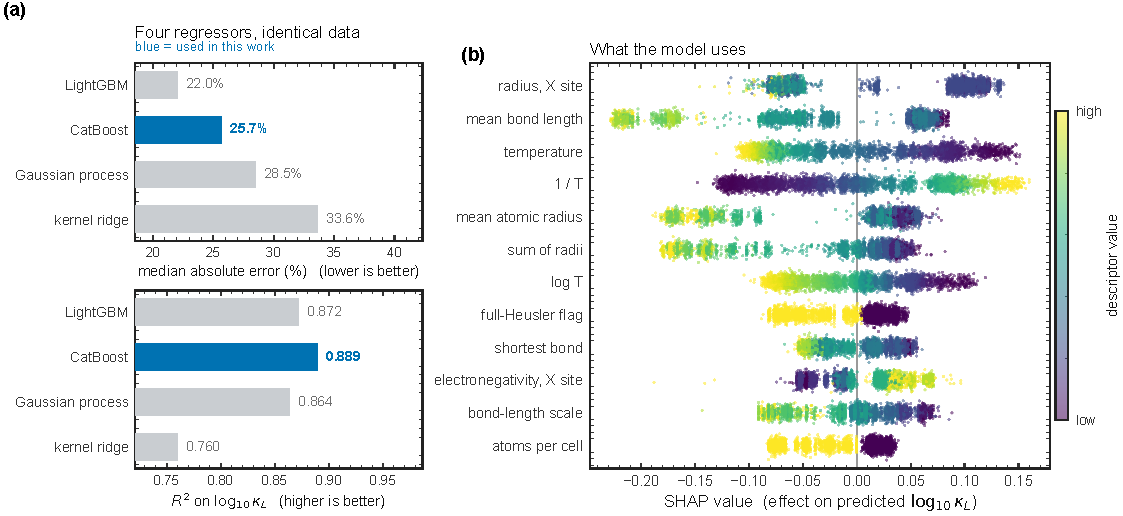
\includegraphics[width=\linewidth]{figures/fig07_model.pdf}
  \caption{\textbf{The regression model: which one, and what it uses.} (a)~Four regressors on
  identical rows and descriptors under grouped cross-validation with whole chemistries held out.
  The two metrics disagree---CatBoost leads on $R^2$, LightGBM on median error---so the blue bar
  marks the model retained, not a winner. (b)~SHAP decomposition of the retained model: for every
  row, how far each descriptor moved the predicted $\log_{10}\kappa_L$, coloured by that
  descriptor's own value. The signs are those thermal transport requires---larger radii, longer
  bonds, more atoms per cell and higher temperature all push $\kappa_L$ down---so the fit rests on
  phonon physics rather than on an artefact of the corpus.}
  \label{fig:model}
\end{figure}

\subsection{Validation, null baselines and prediction intervals}
\label{sec:validation}
\label{sec:nulls}
\label{sec:intervals}

Every figure we report is obtained with the target compound's \emph{entire chemistry} withheld from
training. Compounds are clustered by their most electropositive site and a whole cluster is removed
at once. Compounds sharing the held-out compound's $(\mathrm{Y},\mathrm{Z})$ bonding family but
built on a different X site do remain in training---\num{33} of the \num{38} in-domain compounds
have at least one such relative---so the test measures accuracy for a new X-site substitution
within a known bonding family. It is nonetheless a harder test than removing single compounds,
under which near-duplicates of the target survive in training.

Three precautions make that holdout mean what it says. Any threshold or model choice is made on one
half of the chemistry clusters and evaluated on the other, since selecting on the same data one
reports inflates the result by \SIrange{7.7}{10.3}{pp} depending on the protocol, which we measure
rather than assume. Every reported figure is the median over five model seeds and is quoted with
its across-seed range: the median error moves from \SI{31.0}{\percent} to \SI{40.0}{\percent}
across seeds, so a single-seed figure reports the seed as much as the method, whereas the
within-$2\times$ fraction (\SIrange{81.6}{86.8}{\percent}) and the rank correlation
(\numrange{0.618}{0.675}) are stable, which is why we lean on them. And the two calibration
parameters are themselves refitted with the scored compound's cluster removed; fitting them once on
all \num{38} compounds and scoring the same \num{38} would report \SI{29.7}{\percent} rather than
\SI{31.0}{\percent}.

A method that predicts $\kappa_L$ must beat predictors that use no compound-specific information at
all. We use two: a constant equal to the median measured conductivity of the training compounds,
and a power law $A(T/300)^{q}$ fitted to them. Both are fitted with the same chemistry held out as
the calibration, since a null given less information than the method is not a test of anything.

Intervals are conformal, taken from the out-of-fold residual distribution in logarithmic space
because the error is multiplicative. For a nominal level $\alpha$, over the $m$ held-out compounds
of the declared domain,
%
\begin{equation}
  \delta_\alpha \;=\; \Bigl\{\, \bigl|\log_{10} r_i \bigr| \,\Bigr\}_{(k)},
  \qquad k = \bigl\lceil (m+1)\,\alpha \bigr\rceil,
  \label{eq:conformal}
\end{equation}
%
the $k$-th order statistic of the absolute log-residuals, giving the multiplicative half-width
$10^{\delta_\alpha}$. The $(m+1)$ and the ceiling are both required for finite-sample validity;
the empirical $\alpha$-quantile under-covers at these sample sizes. Coverage is evaluated
leave-one-chemistry-out---the band applied to a held-out cluster is built only from the residuals
of the other clusters---and tracks nominal closely: \SI{50}{\percent} nominal gives
\SI{50.0}{\percent}, \SI{80}{\percent} gives \SI{81.6}{\percent} and \SI{90}{\percent} gives
\SI{92.1}{\percent}, with multiplicative half-widths \num{1.31}, \num{1.92} and \num{2.24}. A
stated interval is therefore a measured frequency rather than an assumption, though on \num{38}
compounds these frequencies carry a binomial uncertainty of roughly \SI{8}{pp} and should be read
as consistent with nominal rather than as precise.

% =============================================================================================
% SECTION 3 -- RESULTS AND DISCUSSION.  Draft 2 -- merge of the former Sections 4, 5 and 6.
%
% Changes of substance from the split version:
%
%   * Every figure now has an introducing sentence in the body. Figs. 2, 4, 5 and 6 previously had
%     none -- Fig. 6 was reached only through another figure's caption, and Fig. 4(c) was never
%     referred to at all.
%   * Fig. 5 has moved to the subsection about the predictions it depicts; it used to sit fifty
%     lines inside the Refusals subsection.
%   * The Fig. 5 and Fig. 6 captions were carrying body content (Fig. 6's 175-word caption held
%     the only description of the conditional tier anywhere in the paper). That material is now in
%     the prose and the captions describe the figures.
%   * One funnel, not two. The 250/234 count and the 181/125 count are the same argument run over
%     two different candidate sets; the second was dropped and the first kept whole.
%   * The Ni-Sb member count is now stated with its set: 29.2 % is over the EIGHT in-domain
%     members, the Fig. 5 envelope is over TEN measured members. Both were correct and the
%     manuscript previously gave them without saying which was which.
%   * The refusal catalogue is a table; it was 600 words of prose.
%
% All labels from the split sections are preserved so existing \ref calls still resolve.
% =============================================================================================

\section{Results and Discussion}
\label{sec:results}

\subsection{Calculations exceed measurements, and the offset is regular}
\label{sec:offset}

Whether a correction is possible at all depends on the offset between calculation and experiment
being systematic rather than idiosyncratic, so we measure it first. For the \num{34} in-domain half
Heuslers carrying both a laboratory measurement and a published transport calculation, the
calculated lattice thermal conductivity exceeds the measured value by a median factor of
\num{1.55}. The excess is not scatter about agreement: it is one-sided, present in every bonding
family, and grows towards low temperature, which is the signature expected when extrinsic
scattering truncates long phonon mean free paths that the calculation allows to propagate freely.

Figure~\ref{fig:offset} shows the offset and its removal. Applying Eq.~\eqref{eq:transfer} with
$c=\num{0.51}$ and $p=\num{0.80}$ fitted over the whole domain---the constants a user of the method
would apply---brings the median ratio from \num{1.55} to \num{1.03}, and raises the fraction of
compound--temperature points within a factor of two of measurement from \SI{72}{\percent} to
\SI{87}{\percent}. The correction therefore centres the population, not merely shrinks it towards
the data. The accuracy figures below are scored under a stricter arrangement, with the
calibration refitted for each held-out chemistry; across those refits $c$ varies only between
\num{0.48} and \num{0.51}.

\begin{figure*}[tp]
  \centering
  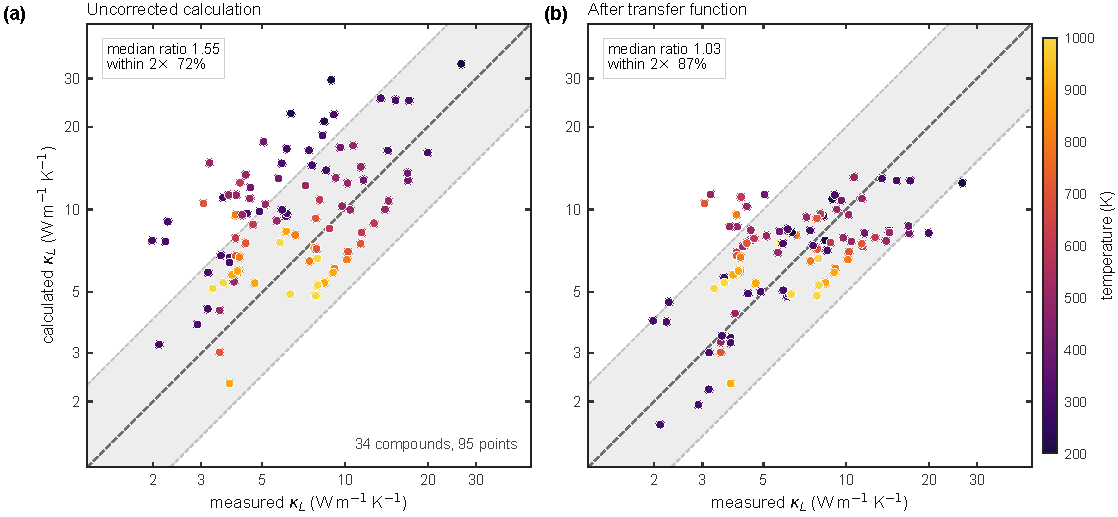
\includegraphics[width=\linewidth]{figures/fig02_offset.pdf}
  \caption{\textbf{Published transport calculations exceed laboratory measurements by a median
  factor of \num{1.55}; the transfer function removes the offset.}
  (a) Calculated against measured $\kappa_L$ for \num{34} in-domain half Heuslers,
  \num{95} compound--temperature points. (b) The same points after Eq.~\eqref{eq:transfer}.
  Shading marks a factor of two. Points are per compound per \SI{100}{\kelvin} bin, not per
  measurement row, since a few heavily sampled compounds (\ce{TiNiSn} \num{753} rows,
  \ce{ZrNiSn} \num{646}) would otherwise dominate.}
  \label{fig:offset}
\end{figure*}

\subsection{Blind-test accuracy}
\label{sec:blind}

Table~\ref{tab:blind} gives the central result. One thing about it should be said before the
numbers rather than after: the predictor being corrected here is the regression model of
Section~\ref{sec:model}, because that is the only one evaluable for all \num{38} compounds. The
route actually deployed for the predictions of Section~\ref{sec:issued} calibrates the
\emph{published} transport calculation instead, and it is more accurate---\SI{27.3}{\percent}
against \SI{31.4}{\percent}, scored separately in Section~\ref{sec:deployed}. Table~\ref{tab:blind}
is therefore the conservative of the two routes.

Across \num{38} half Heuslers spanning \num{18}
chemistry clusters, each predicted with its entire chemistry removed from training, the calibrated
prediction achieves a median absolute error of \SI{33.7}{\percent}---the median over five model
seeds, which individually range from \SI{31.0}{\percent} to \SI{40.0}{\percent}---and places
\SI{86.8}{\percent} of compounds within a factor of two of the measurement. The same model output
without the correction gives \SI{50.5}{\percent} and \SI{65.8}{\percent}. The median ratio of
predicted to measured conductivity is \num{1.00}, against \num{1.32} uncorrected, so the method is
centred and not merely closer. Under the tighter criterion
of \SI{30}{\percent}, the fraction rises from \SI{21.1}{\percent} to \SI{42.1}{\percent}, so two
compounds in five are predicted to within a third.

\begin{table*}[tp]
  \centering
  \caption{Blind-test performance inside the declared domain of applicability. Every compound is
  predicted with its entire chemistry cluster withheld from training, and all nulls are fitted with
  the same chemistry held out as the calibration. Rows that depend on the regression model---the
  first two and the one-parameter ablation---are medians over five model seeds; the nulls, the
  family baseline and the semi-empirical estimates do not depend on the model and are single
  values.}
  \label{tab:blind}
  \begin{tabular}{lcccc}
    \toprule
    & median error & within $2\times$ & within \SI{30}{\percent} & bias \\
    \midrule
    Calibrated (this work)   & \textbf{\SI{33.7}{\percent}} & \textbf{\SI{86.8}{\percent}}
                             & \textbf{\SI{42.1}{\percent}} & \textbf{1.00} \\
    Uncorrected surrogate    & \SI{50.5}{\percent} & \SI{65.8}{\percent}
                             & \SI{21.1}{\percent} & 1.32 \\
    Null: constant $\kappa$  & \SI{44.0}{\percent} & \SI{78.9}{\percent}
                             & \SI{26.3}{\percent} & 1.20 \\
    Null: $A(T/300)^{q}$     & \SI{44.9}{\percent} & \SI{81.6}{\percent}
                             & \SI{26.3}{\percent} & 1.17 \\
    \midrule
    Null: family power law$^{\ddagger}$ & \SI{28.2}{\percent} & \SI{87.1}{\percent}
                             & --- & 1.01 \\
    \midrule
    One parameter, $c$ only  & \SI{44.3}{\percent} & \SI{68.4}{\percent} & \SI{31.6}{\percent} & 0.96 \\
    Slack / Debye--Callaway$^{\dagger}$ & \SI{94.6}{\percent} & \SI{52.4}{\percent} & --- & 1.95 \\
    \bottomrule
    \multicolumn{5}{l}{\footnotesize $^{\dagger}$ published semi-empirical estimates, on the
      \num{21} in-domain compounds that carry one.} \\
    \multicolumn{5}{l}{\footnotesize $^{\ddagger}$ on the \num{31} compounds whose bonding family
      has $\geq 2$ other measured members; see Section~\ref{sec:familynull}.}
  \end{tabular}
\end{table*}

Figure~\ref{fig:curves} shows what this means for individual compounds. Nine are drawn at the
tercile boundaries of the error distribution---the three best, three central and three worst of the
\num{28} in-domain compounds with at least five measured temperatures spanning
\SI{300}{\kelvin}---so the selection is arithmetic rather than editorial. Their median error
(\SI{35.8}{\percent}) matches that of all \num{28} (\SI{33.6}{\percent}), but by construction they
over-represent the tails: their interquartile range is \SI{79}{\percent} against \SI{30}{\percent}
for the full set. The figure is therefore a fair sample of the centre and a deliberately pessimistic
one of the spread. It also shows plainly what the method does not deliver. The predicted curves are
visibly flatter than the measurements in several panels, because Eq.~\eqref{eq:transfer} carries a
single global exponent; the magnitude is corrected, the shape is not.

\begin{figure*}[tp]
  \centering
  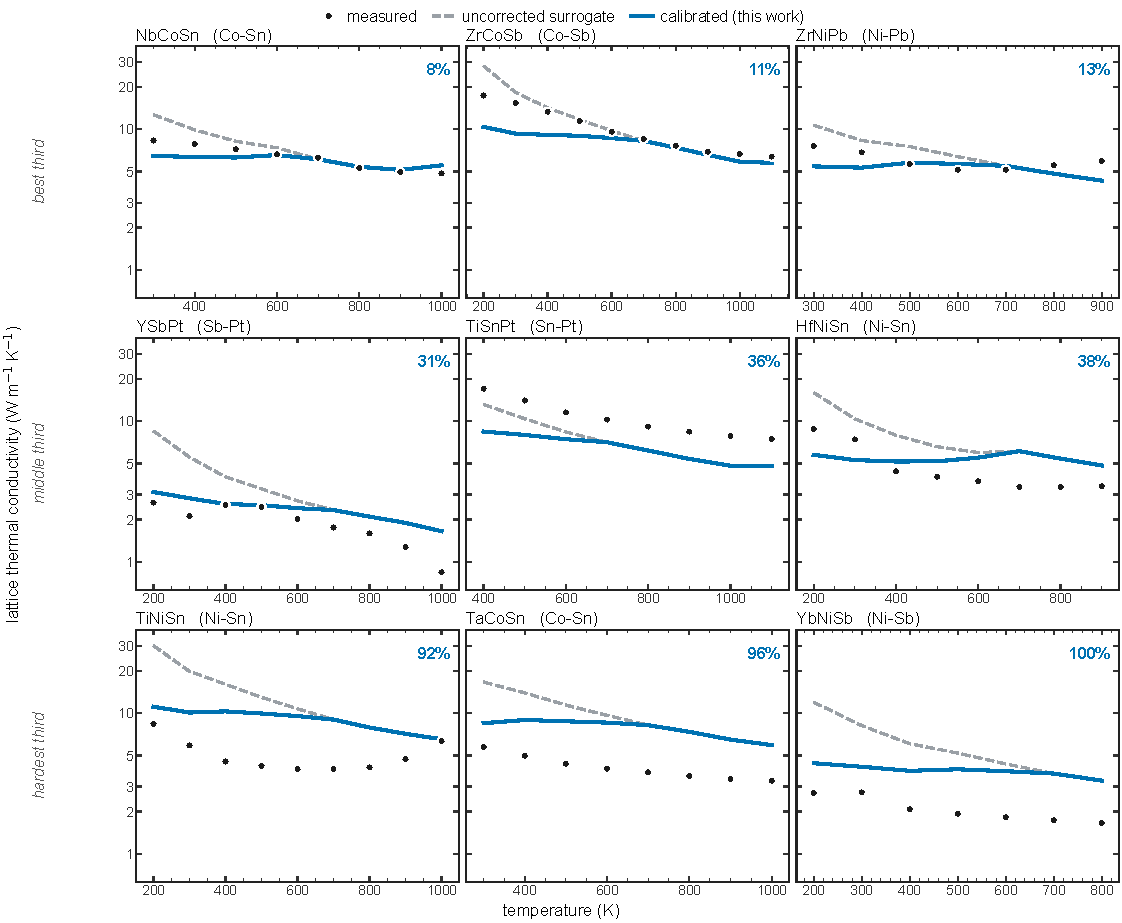
\includegraphics[width=\linewidth]{figures/fig03_curves.pdf}
  \caption{\textbf{The calibrated prediction lands on the measured magnitude; the temperature
  slope is not predicted.} Measured $\kappa_L(T)$ (points), the uncorrected \emph{surrogate}
  (dashed) and the calibrated prediction (solid) for nine in-domain compounds, each with its
  chemistry held out of both the surrogate and the calibration. The dashed curve is the regression
  model's output, not a published transport calculation: the two differ by a median
  \SI{15.4}{\percent} and are scored separately in Section~\ref{sec:deployed}. Rows are the best,
  middle and hardest thirds of the error distribution, drawn at the tercile boundaries;
  per-compound median error is given in each panel.}
  \label{fig:curves}
\end{figure*}

\subsection{Comparison with baselines}
\label{sec:vsnulls}
\label{sec:baselines}

A prediction of $\kappa_L$ earns nothing unless it beats predictors that use no compound-specific
information. Against the two compound-blind nulls of Section~\ref{sec:nulls}, both refitted with
the same chemistry held out as the calibration, the calibrated prediction is better on every metric
in Table~\ref{tab:blind} and closer to the measurement for \SI{65.8}{\percent} of compounds. A paired
Wilcoxon signed-rank test over per-compound errors gives $p=\num{0.050}$ against the constant null
and $p=\num{0.048}$ against the power law, taking the median over seeds; three of the five seeds
clear both nulls at \num{0.05} and two do not. Two qualifications belong with those figures. Both
$p$-values sit at the conventional threshold and would be marginal under a strict correction for
two comparisons, so we present them as evidence rather than proof. And the same test computed over
all \num{51} half Heuslers, before the domain screens are applied, gives $p=\num{0.30}$ and
$p=\num{0.72}$: the separation appears only once the domain is imposed. We regard that as the
expected consequence of removing thirteen compounds in which lattice conduction is not the dominant
channel, and note that the screens were fixed before the validation set was scored. Both numbers
are given.

The rank correlation is the more robust claim---Spearman's
$\rho$ between predicted and measured conductivity is \num{0.65} across the \num{38} compounds
(seed range \numrange{0.618}{0.675}, $p<\num{1e-4}$ for every seed)---and ordering candidates
reliably is what a screening application requires.

Two further comparisons test the method against something better than a null. Both are ablations run
at a single fixed model seed, at which the method's reference figure is \SI{31.0}{\percent} rather
than the seed-median \SI{33.7}{\percent}. Semi-empirical Slack and Debye--Callaway models are the standard cheap route to
$\kappa_L$, and \num{21} of our in-domain compounds carry such an estimate in the literature. On
those \num{21} the published estimates give a median error of \SI{94.6}{\percent} with a bias of
\num{1.95}, against \SI{31.5}{\percent} for the calibrated calculation on the same compounds
(paired Wilcoxon $p=\num{2e-4}$, ours closer for \SI{81}{\percent} of them); no holdout is applied
to the semi-empirical values, which if anything favours them. Dropping our own temperature exponent,
so that $\kappa_L^{\mathrm{expt}} = c\,\kappa_L^{\mathrm{BTE}}$ with a single fitted constant,
raises the median error from \SI{31.0}{\percent} to \SI{45.1}{\percent} and drops the
within-$2\times$ fraction from \SI{86.8}{\percent} to \SI{71.1}{\percent} ($p=\num{0.001}$).
Averaged over seeds the gap is \SI{33.7}{\percent} against \SI{44.3}{\percent}. The exponent is
doing real work, and the method is not a single scale factor with decoration.

\subsection{A stronger baseline: the compound's own bonding family}
\label{sec:familynull}

The nulls above are compound-blind by construction, and the obvious informed alternative is to fit
a power law to the \emph{measured} $\kappa(T)$ of the held-out compound's own
$(\mathrm{Y},\mathrm{Z})$ bonding family and use that. It needs no first-principles calculation, no
regression model and no calibration. It is a strong baseline, and we report it as such: fitted
leave-one-chemistry-out like everything else, it achieves \SI{28.2}{\percent} median error on the
\num{31} in-domain compounds whose family has at least two other measured members
(Table~\ref{tab:populations}). Scored on those same \num{31} our method gives \SI{33.3}{\percent};
the \SI{31.0}{\percent} quoted elsewhere is over all \num{38}, and comparing the two would
understate the gap. Head to
head the difference is not significant (paired Wilcoxon $p=\num{0.22}$) and our method is the closer
of the two for only \SI{42}{\percent} of them. \textbf{On absolute accuracy we do not beat it.}

Two things nonetheless separate the two, and both bear on how the predictions below should be read.
The first is coverage: the family baseline is undefined for \num{7} of the \num{38} in-domain
compounds (\ce{AlVNi}, \ce{NbFeSb}, \ce{TaFeSb}, \ce{YNiBi}, \ce{ZrCoBi}, \ce{ZrNiPb},
\ce{ZrSbIr}), whose families hold too few measured members, whereas a calibrated calculation is
available wherever a calculation is. The second is more fundamental. A family power law returns one
curve per family, so every member receives essentially the same prediction---across our families
the spread between members is only \numrange{1.1}{1.8}---and it therefore cannot order compounds
within a family. Measured against the true ordering, the within-family Spearman correlation is
$-0.90$ for the family baseline and $+0.50$ for the calibrated calculation; in the two families
where we issue predictions the gap is starkest, $+0.93$ against $-0.67$ for \ce{Ni}--\ce{Sb}
($n=8$) and $+0.60$ against $-1.00$ for \ce{Sb}--\ce{Pt} ($n=4$). These correlations rest on three
to eight compounds each and are indicative rather than precise. But within-family ranking is
exactly the task a screening user faces---choosing between \ce{ErSbPt}, \ce{HoSbPt} and
\ce{TmSbPt}, three members of one substitution series, is a within-family problem---and the family
baseline is uninformative for it by construction. The contribution of the calibrated calculation is
not that it predicts the family level better, but that it resolves structure inside a family that a
family-level baseline cannot see.

\subsection{The route that is actually deployed}
\label{sec:deployed}

Table~\ref{tab:blind} is computed on the regression model's output, because that is the predictor
which can be evaluated for all \num{38} compounds. It is not the published transport value: the two
differ by a median of \SI{15.4}{\percent}, and the predictions of Section~\ref{sec:issued} are
issued by calibrating the \emph{published} calculation. That route deserves to be scored on its
own. On the \num{34} in-domain compounds carrying a temperature-matched published transport value,
the uncorrected published calculation gives \SI{71.6}{\percent} median error at a bias of \num{1.72}
and the uncorrected surrogate \SI{66.1}{\percent} at \num{1.66}; calibrated, the surrogate gives
\SI{31.4}{\percent} at \num{1.05} and the published calculation \SI{27.3}{\percent} at \num{1.09}.
The bias of \num{1.72} here and the factor of \num{1.55} quoted in Section~\ref{sec:offset} are the
same offset aggregated two ways: \num{1.55} is the median over the \num{95} compound--temperature
bins of Fig.~\ref{fig:offset}, \num{1.72} the median over the \num{34} compounds. We quote the
binned figure when describing the offset because it is what the figure shows, and the per-compound
figure whenever a compound-level error is being scored.
Two things follow. The uncorrected published calculation is \emph{worse} than the uncorrected
surrogate, so the improvement the transfer function delivers over a raw first-principles value is
larger than Table~\ref{tab:blind} implies, not smaller. And the route we deploy is the better of the
two: where a transport calculation exists, it should be calibrated directly rather than replaced by
a model.

\subsection{Where the method fails, and what did not fix it}
\label{sec:failure}
\label{sec:rejected}

Two failure modes are visible, and both are identifiable in advance. Outside the declared domain
the thirteen excluded compounds have a median error of \SI{105.1}{\percent} against
\SI{29.7}{\percent} inside it, both scored under the single calibration a user would apply
(Mann--Whitney $p=\num{7.5e-3}$); their uncorrected calculations are also far worse and they require
a quite different calibration constant, so they are a distinct population rather than merely harder
examples. Inside the domain, failure sorts by bonding family. Figure~\ref{fig:blind} shows both
effects together with the comparison against the nulls. Grouping in-domain compounds by their
$(\mathrm{Y},\mathrm{Z})$ site pair---the two more electronegative sites, which form the covalent
sublattice that carries the heat---separates the accurate families from the inaccurate:
\ce{Co}--\ce{Sb} (\SI{21.3}{\percent}), \ce{Sb}--\ce{Pt} (\SI{23.2}{\percent}) and
\ce{Ni}--\ce{Sb} (\SI{29.2}{\percent}) are predicted well, while \ce{Co}--\ce{Sn}
(\SI{80.8}{\percent}) and \ce{Bi}--\ce{Pd} (\SI{60.0}{\percent}) are not. The two fail differently,
and the difference decides what we do about them. Every \ce{Co}--\ce{Sn} member still lands within a
factor of two, so its predictions stay inside the band this method claims. \ce{Bi}--\ce{Pd} does
not: only \SI{33}{\percent} of its members are within a factor of two, and its median bias of
\num{0.40} is a systematic \num{2.5}-fold under-prediction rather than scatter. We issue no
predictions in either family. Both rest on three compounds, so these figures indicate where to be
careful rather than measure a failure rate. This grouping is a \emph{post hoc} description of where errors
concentrate: the holdout unit throughout is the X site, not the $(\mathrm{Y},\mathrm{Z})$ pair, so
family members remain in training when a compound is held out and the family error is an
interpolation figure rather than an extrapolation test.

\begin{figure*}[tp]
  \centering
  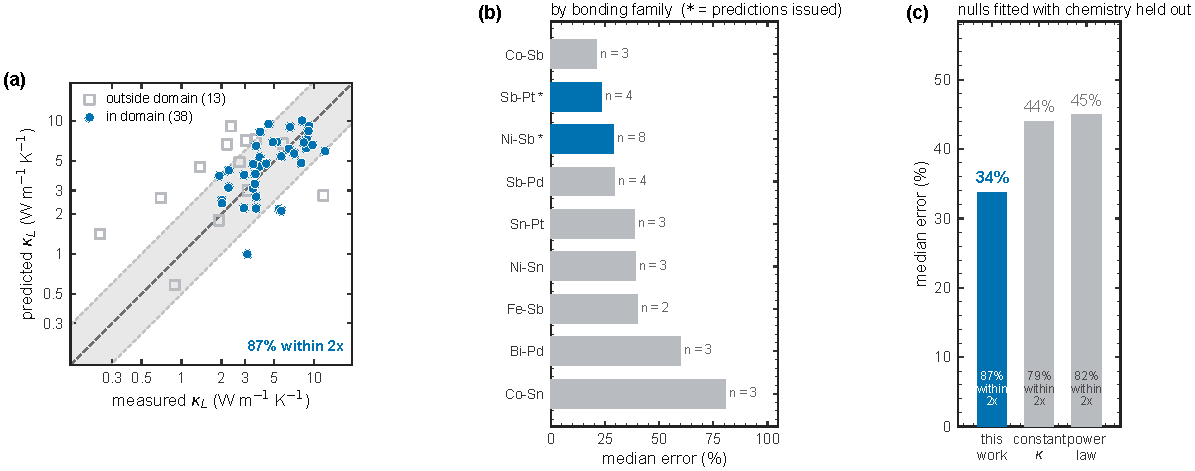
\includegraphics[width=\linewidth]{figures/fig04_blind.pdf}
  \caption{\textbf{\SI{86.8}{\percent} of in-domain compounds are predicted within a factor of
  two.} (a) Predicted against measured $\kappa_L$; open symbols are the thirteen compounds outside
  the declared domain, shown on the same axes. (b) Median error by $(\mathrm{Y},\mathrm{Z})$
  bonding family; starred families are those in which predictions are issued. (c) Against two
  compound-blind nulls, each fitted with chemistry held out; the bar for this work is the
  five-seed median of Table~\ref{tab:blind}, whereas panels (a) and (b) are necessarily drawn from
  a single seed.}
  \label{fig:blind}
\end{figure*}

Five modifications intended to repair these failures were implemented and evaluated under the same
protocol, and none survived it. A hurdle model treating low- and high-conductivity compounds
separately halves the low-$\kappa$ error on calculated labels but changes experimental accuracy by
\SI{-1.3}{pp} ($p=\num{0.84}$). A magnitude term $\kappa^{\beta}$ added to Eq.~\eqref{eq:transfer}
was selected on the design half in 47 of 60 splits and lost on the held-out half. Adding
experimental values to the training set gives \SI{+5.5}{pp} at $p=\num{0.10}$ and is worse on the
transition-metal subset; adding doped-composition data gives no gain at all ($p\geq\num{0.10}$).
Per-family calibration constants are the most interesting failure: the families genuinely do differ
in their raw calculation-to-measurement ratio, but the difference does not transfer, and under
leave-one-chemistry-out a per-family fit gives \SI{31.1}{\percent} against \SI{31.0}{\percent} for
the single global constant ($p=\num{0.22}$, better for only 17 of \num{38} compounds). With two to
four measured members per family, the apparent differences are noise. The single global transfer
function therefore remains the reported method.

\subsection{Predictions for unmeasured compounds}
\label{sec:predictions}
\label{sec:screening}
\label{sec:issued}

We now apply the method to half Heuslers that carry a published transport calculation but no
laboratory measurement, calibrating that published calculation directly. A candidate is carried
forward only if it satisfies every condition below, all evaluated in code at the point the
prediction list is generated, so a compound that fails one cannot reappear in a later regeneration:

\begin{enumerate}
  \item The three domain conditions of Section~\ref{sec:domain}.
  \item \textbf{Not polymorphic.} Which phase forms on synthesis is not ours to assume.
  \item \label{itm:family} \textbf{A validated bonding family:} the $(\mathrm{Y},\mathrm{Z})$
        family must contain at least two compounds predicted correctly against measurement.
        \ce{Bi}--\ce{Pd} is excluded outright on the evidence of Section~\ref{sec:failure}.
  \item \textbf{The label is a transport calculation}, matched on the method string.
  \item \textbf{Inside the family's measured range.} A prediction falling outside the span its own
        family has been measured in is an extrapolation, and is flagged as one rather than issued.
\end{enumerate}

Condition~\ref{itm:family} removes more candidates than the other four together, so it deserves the
most scrutiny. We evaluated it leave-one-out across the \num{36} in-domain compounds for which a
measurement exists, counting the usable anchors in each compound's family \emph{excluding the
compound itself}, which is the situation an unmeasured target actually faces. Compounds whose family
then holds two or more anchors have a median error of \SI{32.3}{\percent} with \SI{96.2}{\percent}
inside a factor of two ($n=\num{26}$); those whose family holds none reach \SI{37.2}{\percent} with
\SI{75}{\percent} inside ($n=\num{8}$). The remaining \num{2} hold exactly one anchor and are the
subject of the relaxation test below. The separation is carried by the within-$2\times$ rate
rather than by the median, and we state it no more strongly than that. Relaxing the threshold from
two anchors to one fails: the two compounds the weaker rule admits have a median error of
\SI{45.5}{\percent} against \SI{32.3}{\percent}. The intuitive alternative---requiring many
chemically similar training compounds---does not survive testing either, since ranking those same
\num{36} compounds by how many calculated compounds share their X site gives a Spearman correlation
with error of $+\num{0.044}$ ($p=\num{0.80}$). What makes a prediction trustworthy here is not the
volume of nearby chemistry but whether an answer has ever been checked in that family.

Five candidates satisfy all five conditions, and they are the complete set rather than a selection.
Enumerating every half Heusler in the corpus that carries a genuine transport calculation between
\SI{150}{\kelvin} and \SI{450}{\kelvin} and has no measurement of its own gives \num{181} compounds,
of which \num{125} clear scope, $\mathrm{VEC}=18$, a cubic record and the radioactivity screen. The
family condition then eliminates almost all the remainder: \num{97} sit in a family with no usable
measured member, \num{9} are \ce{Bi}--\ce{Pd}, \num{8} carry independent calculations that disagree
by a factor of two or more, and \num{1} sits in a family one measurement short. Exactly \num{10}
sit in a validated family, and they are precisely the five predictions and the five flagged cases
below. The binding constraint is therefore not chemistry, not structure and not the availability of
calculations, but the absence of measurements in the families concerned.

Table~\ref{tab:predictions} gives the five, and Fig.~\ref{fig:predictions} draws them inside the
measurements that license them. The transport calculations being calibrated are not ours: they come
from published high-throughput
studies~\cite{li2025highthroug,ohnishi2026database,miyazaki2021machine}, and each predicted value is
that published number multiplied by the transfer function. \ce{ErSbPt} and \ce{HoSbPt} rest on
\num{85} calculated rows each, \ce{TmSbPt}, \ce{GdNiSb} and \ce{TbNiSb} on two or three. The two
families involved are the best predicted in the blind test after \ce{Co}--\ce{Sb}: \ce{Sb}--\ce{Pt}
at \SI{23.2}{\percent} median error over its four in-domain measured members and \ce{Ni}--\ce{Sb} at
\SI{29.2}{\percent} over its eight. Every predicted value falls inside the measured span of its own
family---\SIrange{2.1}{3.8}{\watt\per\meter\per\kelvin} for \ce{Sb}--\ce{Pt} and
\SIrange{2.3}{14.5}{} for \ce{Ni}--\ce{Sb}---so none requires the method to extrapolate beyond
conductivities experiment has already reached in that chemistry. Three of the five (\ce{ErSbPt},
\ce{HoSbPt}, \ce{TmSbPt}) come from a single substitution series in which only the rare-earth site
varies, so the covalent \ce{Sb}--\ce{Pt} sublattice that carries the heat is common to all three and
to the measured members; \ce{GdNiSb} and \ce{TbNiSb} stand in the same relation to the measured
\ce{Ni}--\ce{Sb} compounds. One restriction applies to how they are read: \ce{TmSbPt}, \ce{GdNiSb}
and \ce{TbNiSb} rest on a single calculated temperature, so their values at \SI{600}{\kelvin} and
\SI{900}{\kelvin} would carry only the global exponent and no compound-specific temperature
dependence, and are not quoted. Only \ce{ErSbPt} and \ce{HoSbPt} support a curve.

\begin{table*}[tp]
  \centering
  \caption{Predicted lattice thermal conductivity at \SI{300}{\kelvin} for half Heuslers with a
  published transport calculation and no measurement. All five fall inside the range their own
  bonding family has been measured in, so each is an interpolation within validated chemistry.
  Intervals are conformal (Section~\ref{sec:intervals}).}
  \label{tab:predictions}
  \begin{tabular}{llcccc}
    \toprule
    Compound & Family & $\kappa_L^{\mathrm{BTE}}$ & \textbf{Predicted} &
      \SI{50}{\percent} interval & \SI{90}{\percent} interval \\
    & & \multicolumn{4}{c}{(\si{\watt\per\meter\per\kelvin})} \\
    \midrule
    \ce{TmSbPt} & \ce{Sb}--\ce{Pt} & 5.86 & \textbf{2.99} & 2.28--3.92 & 1.33--6.70 \\
    \ce{HoSbPt} & \ce{Sb}--\ce{Pt} & 7.00 & \textbf{3.57} & 2.73--4.68 & 1.59--8.00 \\
    \ce{ErSbPt} & \ce{Sb}--\ce{Pt} & 7.18 & \textbf{3.66} & 2.79--4.79 & 1.63--8.20 \\
    \ce{GdNiSb} & \ce{Ni}--\ce{Sb} & 8.38 & \textbf{4.27} & 3.26--5.59 & 1.91--9.56 \\
    \ce{TbNiSb} & \ce{Ni}--\ce{Sb} & 9.06 & \textbf{4.62} & 3.53--6.05 & 2.06--10.35 \\
    \bottomrule
  \end{tabular}
\end{table*}

\begin{figure*}[tp]
  \centering
  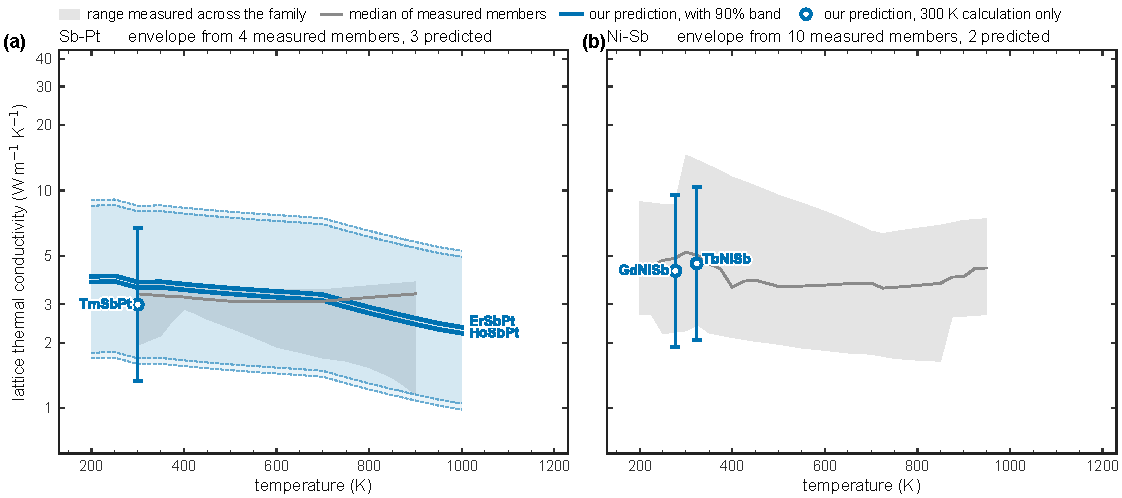
\includegraphics[width=\linewidth]{figures/fig05_predictions.pdf}
  \caption{\textbf{The five issued predictions, drawn inside the measurements that license
  them.} For each validated bonding family the range spanned by that family's measured members is
  shaded, with their median as a grey line, and the predicted compounds are drawn over it in blue
  with their \SI{90}{\percent} conformal band. (a)~\ce{Sb}--\ce{Pt}: envelope from four measured
  members, three predictions. (b)~\ce{Ni}--\ce{Sb}: envelope from ten measured members, two
  predictions. The envelope is drawn over every measured member of the family; the family error
  quoted in the text is over in-domain members only, of which \ce{Ni}--\ce{Sb} has eight.
  \ce{TmSbPt}, \ce{GdNiSb} and \ce{TbNiSb} have a single calculated value at \SI{300}{\kelvin} and
  are drawn as points with their interval; where two coincide their horizontal separation is
  cosmetic. The ordinate is logarithmic because the transfer function is multiplicative.}
  \label{fig:predictions}
\end{figure*}

\subsection{Candidates we decline, and the measurement that would qualify them}
\label{sec:refusals}
\label{sec:whyfive}
\label{sec:novel}

Eleven candidates are declined, and the reasons are as much a result as the five predictions.
Table~\ref{tab:refusals} names them with the condition each fails. Five are flagged---a value
exists and a named check fails---while six are refused outright, and for those six the calibrated
number is not a quantity we are willing to give. The four flagged for falling outside their family's
measured range are not equivalent cases, as the table's margins show: \ce{LaSbPt} and \ce{ScSbPt}
are clear extrapolations, whereas \ce{TmSbPd} and \ce{GdSbPt} miss by less than the factor of
\num{1.33} by which laboratories measuring the same compound routinely disagree. We hold the last
two back as a stated conservatism rather than a validated filter. The boundary is a min--max over
three to five measured compounds and would move if one more were measured, and applied
retrospectively to the \num{16} measured compounds whose families are large enough to test it, the
rule does not separate good predictions from bad (\SI{29.6}{\percent} against \SI{24.8}{\percent},
$p=\num{0.35}$). We keep it because withholding a prediction costs nothing and issuing a wrong one
costs a synthesis, but a reader who weighs that differently has the margins.

\begin{table*}[tp]
  \centering
  \caption{The eleven declined candidates and the condition each fails. Flagged compounds have a
  calibrated value that we do not issue; refused compounds are ones for which we decline to compute
  one.}
  \label{tab:refusals}
  % The third column holds full sentences, so it needs an explicit width. Left as `l' it sets on a
  % single line and runs past the right margin, which is what overlapped the following paragraph.
  \begin{tabular}{llp{0.52\linewidth}}
    \toprule
    Compound & Status & Condition failed \\
    \midrule
    \ce{DySbPd} & flagged  & polymorphic: space group 216 recorded alongside 186 and 194 \\
    \ce{LaSbPt} & flagged  & \num{2.39} below the measured \ce{Sb}--\ce{Pt} floor \\
    \ce{ScSbPt} & flagged  & \num{1.65} above the measured \ce{Sb}--\ce{Pt} ceiling \\
    \ce{GdSbPt} & flagged  & \num{1.24} beyond the nearest measured edge \\
    \ce{TmSbPd} & flagged  & \num{1.09} beyond the nearest measured edge \\
    \midrule
    \ce{TiNiSb} & refused  & $\mathrm{VEC}\neq 18$ \\
    \ce{CrSnPt} & refused  & $\mathrm{VEC}\neq 18$ \\
    \ce{ThNiSn} & refused  & thorium: no training example in the corpus \\
    \ce{ThSnPt} & refused  & thorium: no training example in the corpus \\
    \ce{UNiSn}  & refused  & uranium: no training example in the corpus \\
    \ce{USnPt}  & refused  & uranium: no training example in the corpus \\
    \bottomrule
  \end{tabular}
\end{table*}

Five predictions from a corpus of \num{742} half Heuslers invites the question of where the rest
went, and the answer is not a limitation of the method but a statement about the experimental
literature. Figure~\ref{fig:landscape} sets out everything the method can say and what each
statement is worth, in four tiers. Below the five issued and the eleven declined sits a third tier
of \num{10} compounds that pass every structural and chemical screen but sit in a family with no
usable measured anchor---nine of them \ce{Ni}--\ce{Bi}. These are conditional: the method would
predict them the moment their family acquired two sound measurements, and they are tabulated with
the measurement each waits on in Table~S1 of the supplementary material. Their existence makes the
binding constraint concrete: five laboratory measurements across four bonding families would take
the method from five predictions to nineteen, of which fourteen survive every screen that does not
depend on the new measurement. The ten conditional estimates of Table~S1 are the subset of those
fourteen that carry a calculation at room temperature and can therefore be quoted with a value; the
other four have a transport calculation but not one at \SI{300}{\kelvin}. \ce{Ni}--\ce{Bi} is the most economical, releasing nine predictions
for two measurements, and it is blocked in an instructive way---not by a missing measurement but by
an unusable one. Its sole measured member, \ce{YNiBi}, has a reported $\kappa_L$ that \emph{rises}
with temperature, which lattice conduction cannot do; the measuring authors themselves report the
bipolar contribution responsible~\cite{li2015synthesis}, and a single-parabolic-band Lorenz number
carries no bipolar term, so the electronic part is under-subtracted and the remainder we book as
lattice climbs with temperature. We cannot credit that curve as validation even though our
prediction for it happens to be accurate. Section~S3 of the supplementary material sets out the
literature search behind this case, Section~S2 enumerates the fourteen candidates, and
Section~S5 identifies \ce{Bi}--\ce{Pt} as the most \emph{informative} measurement the corpus points
to, as distinct from the most productive one.

\begin{figure*}[tp]
  \centering
  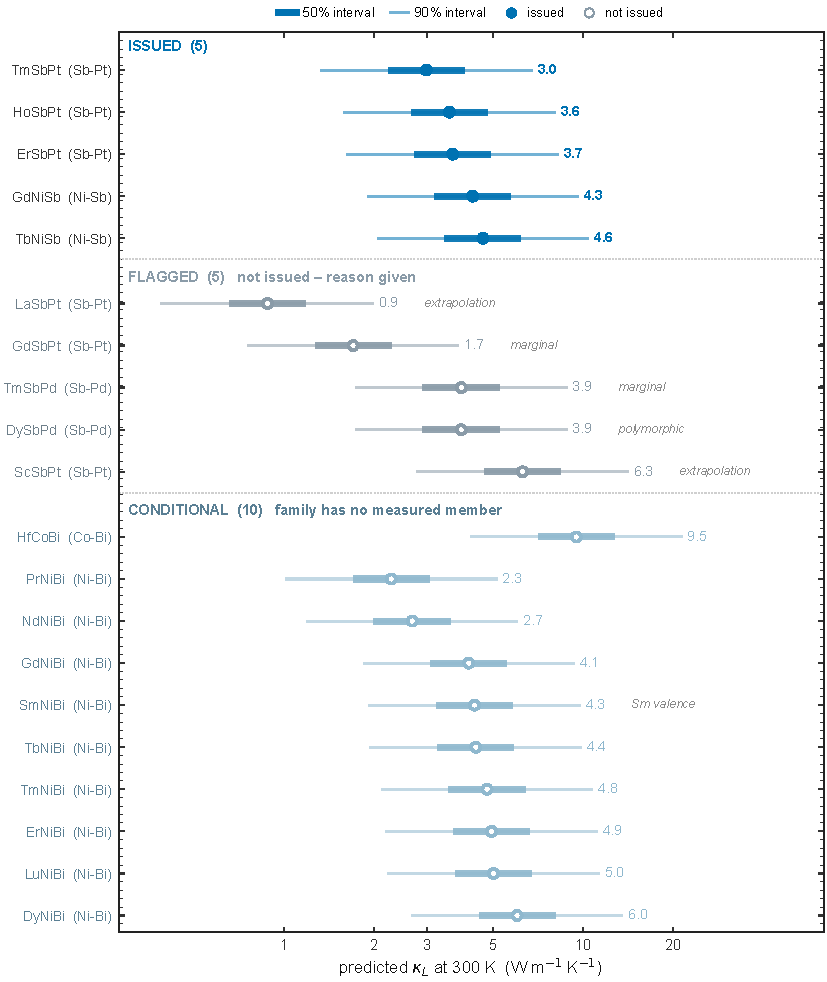
\includegraphics[width=\linewidth]{figures/fig06_landscape.pdf}
  \caption{\textbf{Everything the method can say, and what each statement is worth.} Four tiers,
  ordered by the evidence behind them: \textsc{issued}, the five predictions of
  Table~\ref{tab:predictions}; \textsc{flagged}, five compounds that clear the family test but fail
  one further check; \textsc{conditional}, ten that pass every structural and chemical screen but
  sit in a family with no usable measured anchor; and \textsc{refused}, six declined outright and
  deliberately \emph{not} plotted, since for them the calibrated value is not a quantity we are
  willing to give and drawing it with an interval would assert the opposite. Bars are the
  \SI{50}{\percent} and \SI{90}{\percent} conformal intervals; only the issued tier carries a
  filled prediction marker.}
  \label{fig:landscape}
\end{figure*}

Auditing those candidates surfaced a check we had not been applying anywhere, and it bears on the
predictions we issue as much as on the ones we withhold. Where a compound has been calculated by
more than one group the published values need not agree: across the \num{151} half Heuslers with
two or more independent transport calculations at \SI{300}{\kelvin} the median disagreement is a
factor of \num{1.13}, but the tail reaches \num{18.35}. Two candidates fail on it, and taking the
first available row for one of them, \ce{TiNiPb}, would have issued a prediction of
\SI{55.6}{\watt\per\meter\per\kelvin}---nearly three times the highest value ever measured for any
half Heusler. Independent groups also place the \ce{ErSbPt} and \ce{HoSbPt} calculations \num{1.68}
and \num{1.72} apart; the value we calibrate is mid-range in both cases, but our conformal interval
describes the error of the transfer function and not the spread among its inputs, so for those two
the stated \SI{90}{\percent} band is a lower bound on the true uncertainty.

Separately, we screened compounds with a known crystal structure but no published lattice thermal
conductivity of any kind. One survives: \ce{GaCoMo}, predicted at
\SI{11.3}{\watt\per\meter\per\kelvin} at \SI{300}{\kelvin} (\SI{90}{\percent} interval
\SIrange{5.0}{25.3}{}). Having no published calculation, it must first have one supplied by the
regression model and only then calibrated, so it carries two errors in series by the composite route
that Section~\ref{sec:deployed} shows to be the less accurate. With a chemistry supported by only
three training compounds, we present it as a screening-grade statement---that its conductivity is of
order \SI{10}{\watt\per\meter\per\kelvin} rather than \num{1} or \num{100}---and not as a prediction
on the footing of Table~\ref{tab:predictions}.

\subsection{Limits of the method}
\label{sec:limitations}

Four limitations bound what has been shown beyond those already stated above, and each carries the
number that quantifies it. The first three are recorded where they arise: the temperature slope is
not predicted (Section~\ref{sec:blind}), the family error is an interpolation figure rather than an
extrapolation test (Section~\ref{sec:failure}), and the separation from the nulls sits at the
conventional threshold and does not survive dropping the domain screens
(Section~\ref{sec:vsnulls}). Two quantities complete the first of those: across the \num{33}
in-domain compounds with at least four measured temperatures spanning a factor of \num{1.5} in $T$,
the measured logarithmic slope $\mathrm{d}\ln\kappa_L/\mathrm{d}\ln T$ spans \numrange{-4.78}{0.76}
while the predicted slope spans only \numrange{-0.74}{0.13}, and the rank correlation between them
is $\rho=-\num{0.34}$ ($p=\num{0.05}$)---not merely absent but weakly negative. Compounds governed
by a mechanism with a distinctive temperature signature---bipolar conduction at high
temperature~\cite{li2015synthesis}, or resonant rattling modes~\cite{jana2016the}---are not
distinguished from ordinary ones by anything in our model.

\textbf{The correction is empirical, not a measurement of microstructure.} Its temperature
dependence resembles boundary-limited transport in the Callaway sense~\cite{callaway1959model},
which is why the form was chosen, but the Cauchy--Schwarz argument of
Section~\ref{sec:transfer} caps the log-slope of any single-boundary-length model at $1-c=\num{0.49}$
while our fitted $p=\num{0.80}$ exceeds that ceiling by a factor of \num{1.63}: a quantity that
violates the bound cannot be the boundary term it resembles. The transfer function therefore
absorbs point-defect scattering, site disorder, porosity and interface resistance together with any
boundary contribution. Taken literally its parameters imply a phonon boundary length of order
\SI{44}{\nano\meter}; we report that as a description of the fit, not as a microstructural
measurement, and we make no claim about the grain sizes of the reference specimens.

\textbf{Twelve compounds require the conductivity to be scaled up.} The correction is capped at
unity, encoding the statement that extrinsic scattering cannot raise conductivity above the
perfect-crystal value. Yet for \num{12} of the \num{38} in-domain compounds (\SI{32}{\percent}) the
calculation lies \emph{below} the measurement, with raw ratios as low as \num{0.33}; for those the
functional form cannot help and the residual error is irreducible within this formulation. The cases
concentrate at high temperature---the fraction of matched rows in which the calculation falls below
the measurement rises from \SI{2.9}{\percent} between \SIrange{200}{300}{\kelvin} to
\SI{44.9}{\percent} above \SI{900}{\kelvin}---and two families of explanation fit that pattern
without our being able to separate them. On the calculation side a neglected four-phonon channel
would bite hardest at high temperature and matters in half Heuslers
specifically~\cite{li2024multiphono}, though the dominant approximation in published three-phonon
calculations acts in the opposite direction~\cite{feng2017fourphonon}. On the measurement side,
radiative heat loss inflates laser-flash diffusivity at high temperature~\cite{nishi2020effect} and
bipolar conduction is not removed by a single-parabolic-band Lorenz number~\cite{kim2015characteri}.
We report the pattern rather than assign a cause, and note that it is a property of the reference
data as much as of the method.

\textbf{The calibration is a fitted quantity, not a constant.} Across refits during this work, as
the reference set changed by small amounts, $c$ moved over \numrange{0.37}{0.57}. Any application of
Eq.~\eqref{eq:transfer} to a different compound set should refit rather than adopt our values, and
any comparison with our numbers should carry that range.

\textbf{The reference data carry their own uncertainty.} The measurements against which everything
here is scored are themselves uncertain. Across \num{8545} pairs of independent measurements of the
same compound at the same temperature in our corpus, the median disagreement between laboratories is
a factor of \num{1.33} and the ninetieth percentile a factor of \num{2.00}. A method reporting
\SI{33.7}{\percent} median error is therefore operating near the reproducibility floor of the
field---a \SI{32.5}{\percent} median disagreement between laboratories against our
\SI{33.7}{\percent}---rather than comfortably above it. This is context rather than excuse: it bounds
what any method can demonstrate against this corpus, and it is a further reason to prefer the
rank-ordering claim over the absolute-accuracy one. Twenty-seven of the \num{52} measured compounds
rest on a single publication, so for half the corpus the inter-laboratory spread cannot be assessed
at all.

% =============================================================================================
% SECTION 4 -- CONCLUSIONS.  Draft 2.
%
% Follows the blueprint's conclusion shape: restate the stakes, restate the bottleneck, name the
% need, say what we did, say what validates it, say what it is for, and save the payoff line for
% last. Their conclusion carries counts but NO error statistics -- the numbers live in the
% abstract and the results table, and repeating them here reads as a summary rather than a close.
% Ours keeps two (the offset and the within-2x rate) because they are the claim itself, and drops
% the other four the previous draft restated.
%
% The last sentence is the one thing here that appears nowhere else in the paper.
% =============================================================================================

\section{Conclusions}
\label{sec:conclusions}

Lattice thermal conductivity is the quantity that decides whether a half Heusler is worth
synthesising, and it is also the quantity first-principles transport theory is most often asked to
supply. Because converged calculations are expensive, the field has increasingly reproduced them
with machine-learned surrogates trained on calculated labels---which are what exist in
quantity. The result is a literature of models that predict a calculation accurately and a
measurement only incidentally.

We have shown that the two scales differ by a knowable amount. Across half Heuslers for which both a
published transport calculation and a laboratory measurement exist, the calculation exceeds the
measurement by a median factor of \num{1.55}, one-sidedly and in every bonding family, and the
offset is regular enough to be removed by a closed-form correction with two parameters. Fitting that
correction required a corpus that does not average the two quantities together, so we built one:
\num{52} measured half Heuslers drawn from \num{164} publications alongside \num{289} carrying
transport calculations, every value tiered by the method that produced it.

Validated with each compound's entire chemistry withheld from the model and from the calibration
alike, and inside a domain of applicability declared before the validation set was scored, the
correction places \SI{86.8}{\percent} of held-out compounds within a factor of two of measurement
and orders them reliably. Outside that domain it fails, by a factor we report rather than conceal.
It is a screen and not a curve predictor: it says what a laboratory is likely to measure at a stated
temperature, and its parameters should not be read as a measurement of microstructure. On that basis
we issue five predictions and decline eleven candidates, naming the condition each fails.

The five are falsifiable by a single synthesis each, and we would regard a failure among them as
more informative than the successes. The wider result is that the barrier to predicting more of them
is no longer computational. Fourteen further candidates already carry sound calculations and wait
only on five laboratory measurements across four bonding families---the point at which a
calibration of this kind stops being limited by what has been calculated and starts being limited
by what has been measured.


\section*{Data availability}
\label{sec:data-availability}

The curated corpus, its provenance fields, the prediction list with its refusals, and the code that
generates every figure and number in this paper are available at \repourl. The Starrydata snapshot
used is cited separately so that the corpus can be regenerated exactly.

The measurements analysed here are not ours. Across the whole corpus they were made in \num{198}
publications---of which \num{164} lie behind the \num{52} measured half Heuslers the calibration is
fitted to---and the transport calculations we calibrate come from a further \num{22}. All are
included in the reference list below so that the provenance claim of Section~\ref{sec:dataset} can
be checked rather than taken on trust. Every measured row of the released corpus carries the
digital object identifier of the work it came from; calculated rows drawn from public databases
carry a source URL instead, since those repositories are not identified by DOI.

% ============================================================================================
% PROVENANCE.  GENERATED by scratchpad/gen_provenance.py -- do not hand-edit.
%
% Section 2 claims that every value in the corpus carries an explicit provenance. A reference
% list containing only the works discussed in the text does not demonstrate that claim; it
% leaves the publications the measurements actually come from invisible. These \nocite blocks
% put them into the reference list, which is what makes the claim checkable by a reader.
%
% If the journal objects to the reference count, move this to the supplementary material rather
% than deleting it -- the provenance claim depends on it appearing somewhere.
% ============================================================================================

% --- experimental measurements analysed in this work (198 publications) ---
\nocite{akram2015enhanced,anon2011thermoelec,aversano2020role,bag2020thermoelec,balke2011an}
\nocite{barczak2018impact,barth2009thermoelec,barth2010investigat,barth2010itinerant,berry2017enhancing}
\nocite{berry2017improving,bhardwaj2014improving,bhattacharya2002grain,birkel2012rapid,birkel2013improving}
\nocite{birkel2013influence,buffon2016enhancemen,chauhan2018vanadiumdo,chauhan2019compositio,chauhan2019enhanced}
\nocite{chauhan2019spinodal,chen2018improved,chen2021fast,ciesielski2020thermoelec,delimecodrin2017carrier}
\nocite{ding2016thermoelec,douglas2012enhanced,douglas2014phase,dow2018effect,elkhouly2020transport}
\nocite{ferluccio2018impact,ferluccio2021thermal,fu2012enhanced,gao2020significan,gelbstein2011thermoelec}
\nocite{germond2010thermoelec,gong2019continuous,gong2019effects,graf2010phasesepar,grth2016thermoelec}
\nocite{grytsiv2019thermoelec,han2023strong,hari2020thermoelec,hazama2012thermoelec,he2016enhanced}
\nocite{he2018designing,he2020unveiling,he2026defectcalc,hermet2016lattice,hinterleitner2020stoichiome}
\nocite{hooshmandzaferani2020experiment,huang2004the,huang2015a,huang2017the,huang2018the}
\nocite{huang2019improving,huang2020electron,huang2021point,huang2022discovery,johari2020band}
\nocite{kanemitsu2006transport,katayama2003the,katsuyama2004effect,katsuyama2007thermoelec,katsuyama2010effect}
\nocite{kawaharada2003high,kawaharada2004high,kawaharada2004higha,kawaharada2004highb,kawano2007effect}
\nocite{kim2004enhancemen,kim2007high,kimura2006thermoelec,kimura2006thermoeleca,kimura2008thermoelec}
\nocite{kimura2010vacancy,kirkham2012mmlmath,kurosaki2009effect,laila2020preparatio,landmann2019fabricatio}
\nocite{lei2016microwave,li2010effect,li2013high,li2015synthesis,li2019ntype}
\nocite{li2020titanium,li2024enhancemen,li2025impact,liu2012fabricatio,liu2012lowtempera}
\nocite{liu2025discovery,lkhagvasuren2017improved,lu2009thermoelec,lue2002thermoelec,lue2004offstoichi}
\nocite{lue2004thermal,lue2007thermoelec,lue2008effects,mao2017thermoelec,mastronardi1999antimonide}
\nocite{mato2025starrydata,mena2016miscibilit,miao2026exceptiona,mikami2012thermoelec,mikami2013effect}
\nocite{mikami2015thermoelec,misra2014enhanced,misra2015enhanced,mohamed2020tuning,mondal2018ferromagne}
\nocite{mondal2023thermoelec,morozkin2005thermoelec,mukherjee2020ultralow,mukhopadhyay2018multifunct,muta2005thermoelec}
\nocite{muta2009hightemper,nagai2011preparatio,oestreich2003thermoelec,ojha2024low,ono2006thermoelec}
\nocite{ono2006thermoeleca,ouardi2011transport,ouardi2012electronic,pallecchi2018thermoelec,popescu2024effects}
\nocite{qiu2009enhanced,qiu2010effect,raghuvanshi2021selfdoping,rahul2026linking,ramachandran2018thermoelec}
\nocite{rogl2020halfheusle,sato2021effect,schmitt2015resolving,schrade2017the,schwall2012thermomagn}
\nocite{schwall2018on,sekimoto2005annealing,sekimoto2005thermoelec,sekimoto2005thermoeleca,sekimoto2006lnpdsb}
\nocite{sekimoto2006thermoelec,sekimoto2006thermoeleca,sekimoto2006thermoelecb,sekimoto2006thermoelecc,sekimoto2007highthermo}
\nocite{sekimoto2007thermoelec,serranosnchez2020thermoelec,shastri2020firstprinc,shen2001effects,silpawilawan2017fenbsb}
\nocite{skovsen2010multitempe,sportouch1998observed,synoradzki2019thermal,taranova2019influence,tavassoli2017on}
\nocite{thiem2025thermoelec,toberer2009thermoelec,tseng2017semimetall,uher1999transport,vishwakarma2020compositio}
\nocite{voronin2017preparatio,wang2025enhanced,wei2015thermoelec,wolaska2019enhanced,wu2007thermoelec}
\nocite{wu2009effects,wu2019synergisti,xia2000thermoelec,xia2018enhanced,xie2012increased}
\nocite{xie2012interrelat,xie2014the,xu2020anomalous,yadav2021optical,yadav2022unravellin}
\nocite{yamamoto2017the,yan2020realizing,yang2020enhanced,yang2020identifica,yoshioka2015solid}
\nocite{yousuf2018ternary,yu2010reduced,yu2012high,yuan2017effects,zhang2016synthesis}
\nocite{zhang2021effect,zhao2014synthesis,zhao2018synthesis,zhao2018synthesisa,zhao2021thermoelec}
\nocite{zheng2023symmetrygu,zheng2025boosting,zhou2005effects,zhou2007moderatete,zhu2018discovery}
\nocite{zhu2019discovery,zhu2020enhanced,zou2017band}

% --- transport calculations calibrated in this work (22 publications) ---
\nocite{ali2026comprehens,carrete2014finding,chen2021computatio,deshpande2026a,ding2015examining}
\nocite{ding2016thermoelec,eliassen2017lattice,han2020high,han2023strong,he2019designing}
\nocite{jaishi2021electronic,keshri2020intrinsica,li2025highthroug,miyazaki2021machine,ohnishi2026database}
\nocite{pak2025mapping,raghuvanshi2021selfdoping,rodriguez2023millionsca,shastri2020firstprinc,trans2022lattice}
\nocite{wang2022intrinsic,xue2016laptsb}


% CRediT (Contributor Roles Taxonomy). Elsevier asks for this, and it is the modern answer to the
% ambiguity of author order: it states who did what, so nobody has to infer contribution from
% position in the list. Roles below are drawn from the standard fourteen-term taxonomy -- adjust
% them to what each author actually did, and have each author confirm their own line.
\section*{CRediT authorship contribution statement}

\textbf{Shivam Randive:} Conceptualization, Methodology, Software, Formal analysis,
Data curation, Investigation, Validation, Writing -- original draft.
\textbf{Ojaswini Randive:} Visualization, Writing -- review \& editing.
\textbf{Himanshu Pandey:} Supervision, Resources, Project administration,
Writing -- review \& editing.

\section*{Declaration of competing interest}

The authors declare that they have no known competing financial interests or personal relationships
that could have appeared to influence the work reported in this paper.

% Elsevier requires this as a NAMED statement placed after the competing-interest declaration and
% before the reference list. Check the journal's current author guide for the exact wording it
% asks for, as the policy is revised periodically. Two rules are stable: an AI tool is never an
% author, and use of AI in the RESEARCH (as opposed to the writing) belongs in the Methods --
% which is why the LLM-assisted extraction is described in Section~\ref{sec:dataset} and not here.
\section*{Declaration of generative AI and AI-assisted technologies in the writing process}

During the preparation of this work the authors used Anthropic Claude to draft and revise
manuscript text, to write analysis and figure-generation code, and to audit the manuscript for
internal numerical consistency. Large language models were also used to extract measurements from
primary publications during corpus construction; because that use is part of the research rather
than the writing, it is described in Section~\ref{sec:dataset} together with the safeguards applied
to it. After using these tools the authors reviewed and edited the content as needed and take full
responsibility for the content of the published article.

\section*{Acknowledgements}

\acknowledgementtext

\bibliographystyle{elsarticle-num}
\bibliography{references}

\end{document}
